\documentclass{beamer}
\usetheme{Madrid}
\usefonttheme{professionalfonts}
\usepackage{tikz}
\usepackage{svg}
\usepackage{graphics}
\usepackage{appendixnumberbeamer}
\AtBeginSection[]{
\begin{frame} 
    \frametitle{Contents}
    \tableofcontents[currentsection]
\end{frame}
}
\title[CHY formula]{Scattering of massless particles: scalars, gluons and gravitons}
\subtitle{Freddy Cachazo, Song He, Ellis Ye Yuan}
\author{Su Yingze}
\institute{Nagoya University}
\date[7 23rd 2024]{July 23rd 2024} 
\begin{document}
\frame{\titlepage}
\begin{frame}
    This report is mainly based on the following works
    \begin{itemize}
        \item F. Cachazo, S. He, E.Y. Yuan, arxiv: 1306.6575
        \item F. Cachazo, S. He, E.Y. Yuan, arxiv: 1307.2199
        \item F. Cachazo, S. He, E.Y. Yuan, arxiv: 1309.0885 (Title)
        \item F. Cachazo, S. He, E.Y. Yuan, arxiv: 1412.3479
        \item Z. Bern, J.J.M. Carrasco, H. Johansson, arxiv: 0805.3993
    \end{itemize}
\end{frame}

\section{Why the scattering amplitude is so important?}

\begin{frame}
    \Large \alert{Scattering amplitude is one of the most important concepts in QFT}
    \begin{itemize}
        \pause
        \item It is the bridge connecting experimental data and theoretical prediction.
        \pause
        \item It reveals various properties of theory, such as Lorentz symmetry, localty and unitarity.
        \pause
        \item Some recent work show that scattering amplitude contains many interesting mathematical structures.
    \end{itemize}
\end{frame}
\iffalse
\begin{frame}
    I would like to emphasize two of them, BCFW recursion relations and Amplituhedron.
    \bullet Generally, we would like to consider the scalar theory as the most basic theory in the Quantum field theory. But according to the BCFW, we
            know that amplitudes in sclar theory can not be constructed recursively, but that of more complicated theory --- Yang-Mills, can be completely
            constructed from 3 point amplitudes. So it may give us some new understandings of field theory.

    \bullet It is well known that in the conventional quantum field theory, S-matrix is a deduced physical quantity following
    unitarity and localty. But as the understanding of scatering amplitudes improves, by using the amplituhedron method,
    S-matrix can be constructed directly from a special kind of geometry object and we even have no need to introduce the Lagrangian
    of the specific theory. Also the localty and unitarity can be the outcome from the request of positivity instead of input or previous constraints.
    It may give us some implications about the significance of S-matrix and encourage us to reconstruct the field theory in another way.
    
    \bullet Most of the developments before have made for particular theories like $\mathcal{N}=4$ Super Yang-Mills theory or $\mathcal{N}=8$ Supergravity,
    but this paper gives some hints to the construction of amplitudes for theories with less or no supersymmetry.
\end{frame}
\fi
\begin{frame}{}
    \frametitle{Some developments of amplitudes}
    \begin{itemize}
        \item BCFW recursion relation.
        \begin{equation*}
            \!\!\!\!A_n ~= \!\!\!\!\sum_{\text{diagrams}~I} \hat{A}_\text{L}(z_I) 
            \,\frac{1}{P_I^2}\,
            \hat{A}_\text{R}(z_I)
               ~~=
               \!\!\!\!\sum_{\text{diagrams}~I}
           \raisebox{-5.5mm}{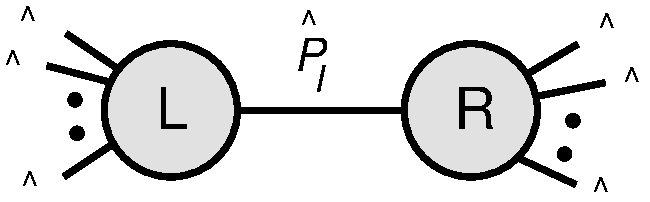
\includegraphics[height=1.4cm]{recrel1.pdf}}
           \,.
        \end{equation*}
        \item Dual superconformal symmetry of $\mathcal{N}=4$ Super Yang-Mills amplitude.
        \item Generalized unitarity
        \item Positive geometry and Amplituhedron.
        \item \dots
    \end{itemize}
    \begin{figure}
        \centering
        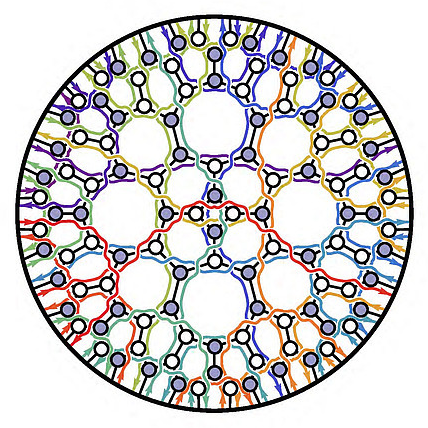
\includegraphics[width=0.25\linewidth]{Grassmannian.png}
        \caption{Positive Grassmanian}
    \end{figure}
\end{frame}
\begin{frame}
    

\tikzset{every picture/.style={line width=0.75pt}} %set default line width to 0.75pt        

\begin{tikzpicture}[x=0.75pt,y=0.75pt,yscale=-1,xscale=1]
%uncomment if require: \path (0,300); %set diagram left start at 0, and has height of 300

%Straight Lines [id:da04992460244937069] 
\draw    (116,79) -- (116.49,163) ;
\draw [shift={(116.5,165)}, rotate = 269.67] [color={rgb, 255:red, 0; green, 0; blue, 0 }  ][line width=0.75]    (10.93,-3.29) .. controls (6.95,-1.4) and (3.31,-0.3) .. (0,0) .. controls (3.31,0.3) and (6.95,1.4) .. (10.93,3.29)   ;
%Straight Lines [id:da7393833245286348] 
\draw    (218,134) -- (343.5,134) ;
\draw [shift={(345.5,134)}, rotate = 180] [color={rgb, 255:red, 0; green, 0; blue, 0 }  ][line width=0.75]    (10.93,-3.29) .. controls (6.95,-1.4) and (3.31,-0.3) .. (0,0) .. controls (3.31,0.3) and (6.95,1.4) .. (10.93,3.29)   ;
%Straight Lines [id:da6514784763465036] 
\draw    (447,76) -- (447.49,160) ;
\draw [shift={(447.5,162)}, rotate = 269.67] [color={rgb, 255:red, 0; green, 0; blue, 0 }  ][line width=0.75]    (10.93,-3.29) .. controls (6.95,-1.4) and (3.31,-0.3) .. (0,0) .. controls (3.31,0.3) and (6.95,1.4) .. (10.93,3.29)   ;
%Straight Lines [id:da8109804852164224] 
\draw    (257,265) -- (320.5,265) ;
\draw [shift={(322.5,265)}, rotate = 180] [color={rgb, 255:red, 0; green, 0; blue, 0 }  ][line width=0.75]    (10.93,-3.29) .. controls (6.95,-1.4) and (3.31,-0.3) .. (0,0) .. controls (3.31,0.3) and (6.95,1.4) .. (10.93,3.29)   ;

% Text Node
\draw (79,46) node [anchor=north west][inner sep=0.75pt]   [align=left] {$\mathrm{Lagrangian}$};
% Text Node
\draw (86,178) node [anchor=north west][inner sep=0.75pt]   [align=left] {$\mathrm{S-matrix}$};
% Text Node
\draw (391,49.4) node [anchor=north west][inner sep=0.75pt]    {$\mathrm{Amplituhedron}$};
% Text Node
\draw (417,173) node [anchor=north west][inner sep=0.75pt]   [align=left] {$\mathrm{S-matrix}$};
% Text Node
\draw (94,256) node [anchor=north west][inner sep=0.75pt]   [align=left] {$\mathrm{Positivity}$ of $\mathrm{geometry}$ };
% Text Node
\draw (339,255) node [anchor=north west][inner sep=0.75pt]   [align=left] {$\mathrm{Unitarity}$ and $\mathrm{Localty}$};


\end{tikzpicture}

\end{frame}

\section{CHY Formula}
\begin{frame}
    \frametitle{Motivation}
    %Most of the developments of amplitudes before have made for some specific theories, like N=4 super yang-mills theory and N=8 supergravity.
    %The natural question is that what is the space of all field theories whose tree level S-matrix can be expressed in a compact form? 
    \begin{itemize}
        \item Compact form of amplitudes for sclar, pure Yang-Mills and gravity theories in any spacetime dimension.
        %The author introduce a compact form of tree level amplitudes for three different theories, colored scalar theory, pure Yang-Mills and Einstein gravity.
        %The concrete form of this formula implies that there is a relation between these three theories, and it may give some new insights of the connection between gravity and gauge theory.
        \item A special amplitude --- Double partial amplitude
        %Because of the special color structure of this scalar theory, the authors proposed a easy method to compute all scalar tree amplitudes, and then pure Yang-Mills and gravity can also be done using similar methods.
        \item BCJ double copy at tree level
        %In terms of this construction of amplitudes, it is easy to obtain the BCJ double copy relation.
        \item Related to other theories, such as EYM, EM, NLSM and so on.
        %In the following paper of these authors, by introducing some special operations which performed on the integrand of CHY formula, they give some relations between other theories.   
        \item One-loop corrections to scattering amplitudes of scalars and gauge bosons can be obtained from tree amplitudes in one higher dimension. 
    \end{itemize}
\end{frame}
\begin{frame}
    \frametitle{Scattering equations}
    % In the Witten-RSV formulation, tree-level field theory amplitudes are given as integrals that localize on generic spheres.
    It has been proposed that there is connection between the scattering data of n massless particles and the n-punctured sphere from a rational map
    \begin{equation*}
        k_\mu^a=\frac{1}{2\pi i}\oint_{|z-\sigma_a|}dz\frac{p^\mu(z)}{\prod ^n_{b=1}(z-\sigma_b)}
    \end{equation*}
 
    To discribe the n-punctured sphere more properly, we can introduce the Riemann sphere as
    \begin{equation*}
        \mathbb{CP}^1\cong \mathcal{S}^2\cong \mathbb{C}\cup\{\infty\}
    \end{equation*}
    each $\sigma_a$ represents a puncture located in the Riemann sphere.
   
\end{frame}
\iffalse
and n-punctured Riemann sphere can be discribed by $SL(2,\mathbb{C})$ affine coordinates ${\sigma_1,\sigma_2,\ldots,\sigma_n}$, that is to say we have a equvilance relation
\begin{align*}
    \{\sigma_1,\sigma_2,\ldots,\sigma_n\}\sim\{\psi(\sigma_1),\psi(\sigma_2),\ldots,\psi(\sigma_n)\},\\\psi(\sigma):=\frac{\alpha\sigma+\beta}{\gamma\sigma+\delta},\quad\alpha,\beta,\gamma,\delta\in\mathbb{C},\alpha\delta-\beta\gamma=1
\end{align*}
because of the redundancy of $\mathrm{SL}(2,\mathbb{C})$, only $n-3$ of them are independent.
\fi
\begin{frame}
    From this map, we can easily obtain the main ingredients of this report \\
    

    \begin{block}{\textcolor{red}{Scattering equations}}
        \begin{equation*}
            \sum_{b\neq a } \frac{s_{ab}}{\sigma_a-\sigma_{b}}=0,\qquad a\in \{1,\dots,n\}
        \end{equation*}
    \end{block}
    \pause
    It can be shown that this equation is invariant under the $SL(2,\mathbb{C})$ transformation, that is to say
    \begin{align*}
        \{\sigma_1,\sigma_2,\ldots,\sigma_n\}\sim\{\psi(\sigma_1),\psi(\sigma_2),\ldots,\psi(\sigma_n)\},\\\psi(\sigma):=\frac{\alpha\sigma+\beta}{\gamma\sigma+\delta},\quad\alpha,\beta,\gamma,\delta\in\mathbb{C},\alpha\delta-\beta\gamma=1
    \end{align*}
    so only $\alert{n-3}$ of these equations are independent, and it has also been proved that these equations have $\alert{(n-3)!}$ solutions in any dimension. 
    \begin{equation*}
        \sum_{b\neq a } \frac{s_{ab}}{\sigma_a-\sigma_{b}}=0,\quad a\in \{4,5,\dots,n\}\quad and\quad  \sigma_1\rightarrow\infty,\sigma_2=0,\sigma_3=1
    \end{equation*}
\end{frame}
\iffalse
\section{CHY Formula}
\begin{frame}{Scattering equations}
    It has benn proposed that there is connection between the scattering data of n massless particles and the n-punctured sphere from a rational map
    \begin{equation*}
        k_\mu^a=\frac{1}{2\pi i}\oint_{|z-\sigma_a|}dz\frac{p^\mu(z)}{\prod ^n_{b=1}(z-\sigma_b)}
    \end{equation*}
 
    To discribe the n-punctured sphere more properly, we can introduce the Riemann sphere as
    \begin{equation*}
        \mathbb{CP}^1\cong \mathcal{S}^2\cong \mathbb{C}\cup\{\infty\}
    \end{equation*}
    and n-punctured Riemann sphere can be discribed by $SL(2,\mathbb{C})$ affine coordinates ${\sigma_1,\sigma_2,\ldots,\sigma_n}$, that is to say we have a equvilance relation
    \begin{align*}
        \{\sigma_1,\sigma_2,\ldots,\sigma_n\}\sim\{\psi(\sigma_1),\psi(\sigma_2),\ldots,\psi(\sigma_n)\},\\\psi(\sigma):=\frac{\alpha\sigma+\beta}{\gamma\sigma+\delta},\quad\alpha,\beta,\gamma,\delta\in\mathbb{C},\alpha\delta-\beta\gamma=1
    \end{align*}
    because of the redundancy of $\mathrm{SL}(2,\mathbb{C})$, only $n-3$ of them are independent.
\end{frame}
\begin{frame}
    From this map, we can easily obtain the main ingredients of this report \\
    

    \begin{block}{\textcolor{red}{Scattering equations}}
        \begin{equation*}
            \sum_{b\neq a } \frac{s_{ab}}{\sigma_a-\sigma_{b}}=0,\qquad a\in \{1,\dots,n\}
        \end{equation*}
    \end{block}
    It has been proved that the number of solutions in any dimension is $\alert{(n-3)!}$, and only \alert{$n-3$} of the equtions are independent, so we can rewrite the scattering equations as following 
    \begin{equation*}
        \sum_{b\neq a } \frac{s_{ab}}{\sigma_a-\sigma_{b}}=0,\quad a\in \{4,5,\dots,n\}\quad and\quad  \sigma_1\rightarrow\infty,\sigma_2=0,\sigma_3=1
    \end{equation*}
\end{frame}
\fi

\begin{frame}
    \frametitle{Attempt to construct S-matrix --- Towards CHY}
    %Thanks to the excellent properties of scattering equations, it is very tempting to propose that the solutions
    %to scattering equations should be used to construct scattering amplitudes.
    The first two constructed are YM and gravity amplitudes in any dimensions
    \begin{align*}
        M_n^{\mathrm{YM}}&=\int\frac{d^n\sigma}{\mathrm{vol\,SL}(2,\mathbb{C})}\prod_a{'}\delta\bigg(\sum_{b\neq a}\frac{s_{ab}}{\sigma_{ab}}\bigg)\frac{E_n(\{k,\epsilon,\sigma\})}{\sigma_{12}\dots\sigma_{n1}},\\
        M_n^{\mathrm{gravity}}&=\int\frac{d^n\sigma}{\mathrm{vol\,SL}(2,\mathbb{C})}\prod_a{'}\delta\bigg(\sum_{b\neq a}\frac{s_{ab}}{\sigma_{ab}}\bigg)E_n(\{k,\epsilon,\sigma\})^2
    \end{align*}
    \pause
    The delta function is defined as following
    \begin{equation*}
        \frac{d^n\sigma}{\mathrm{vol\,SL}(2,\mathbb{C})}{:}=\prod_{c\neq p,q,r}d\sigma_c(\sigma_{pq}\sigma_{qr}\sigma_{rp})
    \end{equation*}
    \begin{equation*}
        \prod_{a}{}^{\prime}\delta{\left(\sum_{b\neq a}\frac{s_{ab}}{\sigma_{ab}}\right)}{:}=\sigma_{ij}\sigma_{jk}\sigma_{ki}\prod_{a\neq i,j,k}\delta{\left(\sum_{b\neq a}\frac{s_{ab}}{\sigma_{ab}}\right)}
    \end{equation*}
\end{frame}

\begin{frame}
    \frametitle{The form of measure}
    The measure can be computed %the n-3 integral can be completely determined by n-3 delta function
    \begin{equation*}
            \boxed{
            \sum_{\{\sigma\}\in\mathrm{solutions}}\frac{(\sigma_{pq}\sigma_{qr}\sigma_{rp})(\sigma_{ij}\sigma_{jk}\sigma_{ki})}{|\Phi|_{pqr}^{ijk}}}
    \end{equation*}
    where the determinant is that of the following Jacobbi matrix
    \begin{equation*}
        \Phi_{ab}\equiv\partial\left(\sum_{c\neq a}\frac{s_{ac}}{\sigma_a-\sigma_c}\right)/\left(\partial\sigma_b\right)=\begin{cases}\frac{s_{ab}}{(\sigma_a-\sigma_b)^2},&a\neq b,\\-\sum_{c\neq a}\Phi_{ac}, &a=b\end{cases}
    \end{equation*}
    \pause
    Usually we take the notation as following
    \begin{equation*}
        \boxed{
        \det{'}\Phi:=\frac{|\Phi|_{pqr}^{ijk}}{(\sigma_{pq}\sigma_{qr}\sigma_{rp})(\sigma_{ij}\sigma_{jk}\sigma_{ki})}}
    \end{equation*}
\end{frame}

\begin{frame}
    \frametitle{The form of integrand}
    In order to present the explict form of $E_n(\{k,\epsilon,\sigma\})$, first define the following $2n\times2n$ antisymmetric matrix 
    \begin{equation*}
        \Psi=\begin{pmatrix}
            A & -C^T \\
            C & B 
        \end{pmatrix}
    \end{equation*}
    where $A,B$ and $C$ are $n\times n$ matrices, defined as 
    \begin{equation*}
        A_{ab}=\begin{cases}\frac{s_{ab}}{\sigma_a-\sigma_b}&a\neq b,\\0&a=b,\end{cases} \quad 
        B_{ab}=\begin{cases}\frac{\epsilon_a \cdot \epsilon_b}{\sigma_a-\sigma_b}&a\neq b,\\0&a=b, \end{cases} \quad
    \end{equation*}
    \begin{equation*}
        C_{ab}=\begin{cases}\frac{\epsilon_a\cdot k_b}{\sigma_a-\sigma_b}&a\neq b,\\-\sum_{c\neq a}\frac{\epsilon_a\cdot k_c}{\sigma_a-\sigma_c}&a\neq b.\end{cases}
    \end{equation*}
\end{frame}
\begin{frame}
    %The first important observation is that while the Pfaffian of $\Psi$ is 0, but after removing any rows $i,j$ and colums $i,j$
    %with $1\leq i< j\leq n$, the new matrix $\Psi_{ij}^{ij}$ have nonzero Pfaffian and we define the corresponding reduced Pfaffian as 
    %The Pfaffian of $\Psi$ is 0, but aftering removing any two rows and colums $i,j$ with $1\leq i< j\leq n$, 
    %the new matrix $\Psi_{ij}^{ij}$ have nonzero Pfaffian and we define the corresponding reduced Pfaffian as
    Because the $\mathrm{Pfaffian}$ of $\Psi$ equals to 0, so it is necessary to define the reduced $\mathrm{Pfaffian}$ like 
    \begin{equation*}
            \boxed{
            \mathrm{Pf}^{\prime}\Psi:=\frac{(-1)^{i+j}}{(\sigma_i-\sigma_j)}\mathrm{Pf}(\Psi_{ij}^{ij})}
    \end{equation*}
    where $1\leq i< j\leq n$.
    \\ \hspace*{\fill}\\
    It can be proved that the reduced Pfaffian is invariant under permutaion of \alert{particle labels}.
    \pause
    \begin{alertblock}{$\mathrm{Pfaffian}$}
        Pfaffian is defined for antisymmetric matrix, usually in two ways as following
        \begin{itemize}
            \item  $\mathrm{Pf}(A)^2=\det A$
            \item  $\mathrm{Pf}(A)=\frac{1}{2^n n!}\sum_{\sigma \in S_{2n}}sgn(\sigma)\prod_{i=1}^n a_{\sigma_{(2i-1)},\sigma(2i)}$
        \end{itemize}
    \end{alertblock}
\end{frame}
\begin{frame}
    Write down the proposal
    \alert{
    \begin{equation*}
        E_n(\{k,\epsilon,\sigma\})=\mathrm{Pf}^\prime \Psi(k,\epsilon,\sigma)
    \end{equation*}}
    Combine the measure and integrand, we conclude the formula for the tree-level S-matrix of Yang-Mills in any dimension
    \begin{equation*}
        M_n^{\mathrm{YM}}=\frac{1}{\mathrm{vol\,SL}(2,\mathbb{C})}\int\frac{d^n\sigma}{\sigma_{12}\cdots\sigma_{n1}}\prod_{a}{}^{\prime}\delta{\left(\sum_{b\neq a}\frac{s_{ab}}{\sigma_{ab}}\right)}\mathrm{Pf}^{\prime}\Psi
    \end{equation*}
    and gravity amplitudes by using KLT construcion
    \begin{equation*}
        M_n^{\mathrm{gravity}}=\frac{1}{\mathrm{vol\,SL}(2,\mathbb{C})}\int d^n\sigma\prod_{a}{}^{\prime}\delta{\left(\sum_{b\neq a}\frac{s_{ab}}{\sigma_{ab}}\right)}\mathrm{Pf}^{\prime}\Psi\mathrm{Pf}^{\prime}\Psi
    \end{equation*}
\end{frame}
\begin{frame}
    We can also write the amplitude in another form
    \begin{equation*}
        M_n^{\mathrm{YM}}=\sum_{\{\sigma\}\in\mathrm{solutions}}\frac{1}{\sigma_{12}\cdots\sigma_{n1}}\frac{\mathrm{Pf}^\prime \Psi(k,\epsilon,\sigma)}{\det{'}\Phi}
    \end{equation*}
    \begin{equation*}
        M_n^{\mathrm{gravity}}=\sum_{\{\sigma\}\in\mathrm{solutions}}\frac{\det{'}\Psi(k,\epsilon,\sigma)}{\det{'}\Phi}
    \end{equation*}
    where we use the property of Pfaffian $\det{'}\Psi(k,\epsilon,\sigma)=\mathrm{Pf}^\prime \Psi(k,\epsilon,\sigma)$\\$\times \mathrm{Pf}^\prime \Psi(k,\epsilon,\sigma)$.
\end{frame}
\begin{frame}
    \frametitle{Consistency check}
    \begin{itemize}
        \item \alert{Gauge invariance}\\
        % The gauge invariance is just the statement that the amplitudes vanishes when we replace any polarization vector by the corressponding momentum vector.
        If we replace the ith polariazation vector $\epsilon_i^\mu$ by momentum $k_i^\mu$, we find that
        \begin{equation*}
            C_{ii}=-\sum_{c\neq i}\frac{\epsilon_i\cdot k_c}{\sigma_i-\sigma_c} \to -\sum_{c\neq i}\frac{k_i\cdot k_c}{\sigma_i-\sigma_c}=0
        \end{equation*}
        It is easy to discover that the $i$th and $i+n$ th colums become identical, so the determinat becomes 0 and then Pfaffian becomes 0.
        \pause
        \item \alert{Soft limit}\\
        Using a special property of Pfaffian
        \begin{equation*}
            \mathrm{Pf} (E)=\sum_{q=1}^{2n}(-1)^q e_{pq}\mathrm{Pf}(E^{pq}_{pq})
        \end{equation*}
        we find the amplitude in the soft limit is 
        \begin{equation*}
            A_n\to\left(\frac{\epsilon_n\cdot k_{n-1}}{k_n\cdot k_{n-1}}+\frac{\epsilon_n\cdot k_1}{k_n\cdot k_1}\right)A_{n-1}
        \end{equation*}
    \end{itemize}
\end{frame}

%Since the Yang-Mills and gravity tree-level amplitudes can be written in a compact form, it is tempting to generalize it to other theories.
\begin{frame}
    \frametitle{CHY form for 3 specific theory}
    Both formulas above can be written in this simplest form % This formula comes from the subsquent work of the same authors.
    \alert{
        \begin{equation*}
            \!\!\!\!\mathcal{M}^{(s)}\!=\!\!\!\int\frac{d^n\sigma}{\mathrm{vol\,SL}(2,\mathbb{C})}\prod_a{'}\delta\bigg(\sum_{b\neq a}\frac{s_{ab}}{\sigma_{ab}}\bigg)
            \!\!\!\left(\frac{\mathrm{Tr}(T^{a_1}\dots T^{a_n})}{(\sigma_{12})\dots (\sigma_{n1})}+\dots\right)^{(2-s)}\!{(\mathrm{Pf}^\prime\Psi)}^s
        \end{equation*}}
    with $s=1$ for Yang-Mills and $s=2$ for gravity.
    \\ \hspace*{\fill}\\
    \pause
    \begin{equation*}
        \mathcal{M}^{(s)} \text{ as \alert{definition of S-matrix for spin s particles}}
    \end{equation*}
    \begin{equation*}
        s=0\quad\to \quad \text{There should be a corresponding scalar theory}
    \end{equation*}
\end{frame}
\begin{frame}
    %In order to get more general case, the gravity amplitudes actually can be modified to the product of two different Pfaffians,each with own choice of polariazation vector
    The general case is that we can choose different polarization vector like 
    \begin{equation*}
        \left(\mathrm{Pf}^\prime \Psi(k,\epsilon,\sigma)\right)^2\to\mathrm{Pf}^\prime \Psi(k,\epsilon,\sigma)\mathrm{Pf}^\prime \Psi(k,\tilde{\epsilon},\sigma)
    \end{equation*}
    actually it gives amplitudes with gravitons coupled to dilatons and B-fields.
    \\ \hspace*{\fill}\\
    \pause
    For the case $s=0$, the similar consequence is 
    \begin{equation*}
        \left(\frac{\mathrm{Tr}(T^{a_1}T^{a_2}\dots T^{a_n})}{(\sigma_{12})\dots (\sigma_{n1})}\right)^2\to\left(\frac{\mathrm{Tr}(T^{a_1}\dots T^{a_n})}{(\sigma_{12})\dots (\sigma_{n1})}\right)
        \left(\frac{\mathrm{Tr}(\tilde{T}^{b_1}\dots \tilde{T}^{b_n})}{(\sigma_{12})\dots (\sigma_{n1})}\right)
    \end{equation*}
    while the original color group is $U(N)$, the new factors are the product of two different color group \alert{$U(N)\times U(\tilde{N})$}.
\end{frame}
\begin{frame}
    The simplest possibility is the theory with only cubic interaction
    \begin{equation*}
        -f_{abc}\tilde{f}_{a^\prime b^\prime c^\prime}\phi^{aa^\prime}\phi^{bb^\prime}\phi^{cc^\prime}
    \end{equation*}
    usually called \alert{bi-adjoint} scalar theory.
    \\ \hspace*{\fill}\\
    All of above leads to the conclusion that the factors 
    \begin{equation*}
        \mathcal{C}_{U(N)}\equiv \sum_{\sigma\in S_n/Z_n}\left(\frac{\mathrm{Tr}(T^{a_1}T^{a_2}\dots T^{a_n})}{(\sigma_{12})\dots (\sigma_{n1})}\right)\quad \mathrm{and} \quad E_\epsilon\equiv\mathrm{Pf}^{'}\Psi(\epsilon)
    \end{equation*}
    are interchangeable and this is a Color-Kinematics corresopondence which is valid for individual solutions to scattering equations.
   
\end{frame}

\begin{frame}
    The connection of amplitudes between 3 theories can be described by the following diagram 
    \begin{figure}[htb]
        \centering
        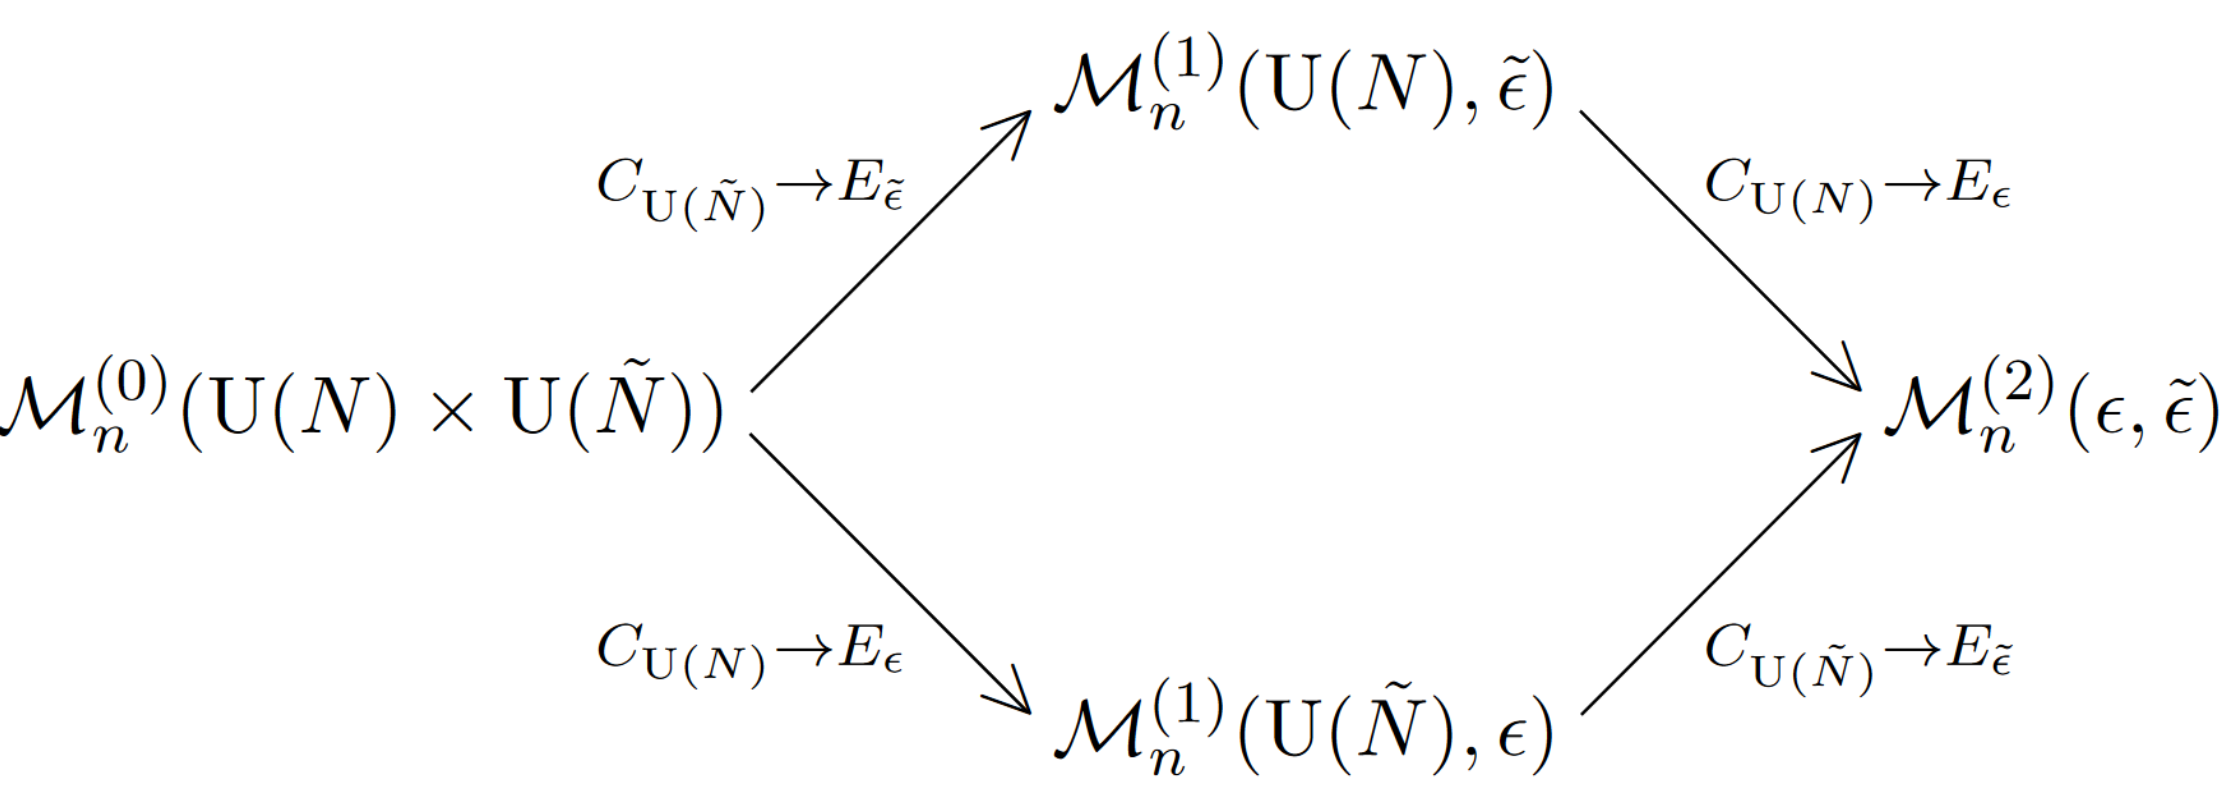
\includegraphics[width=1\linewidth]{main.png}
    \end{figure}
\end{frame}
\begin{frame}
    \frametitle{Double partial amplitudes}
    Because there are two color indices in this sclar theory, so it can be anticipated that the amplitude
    have double trace decomposition structure
    \begin{align*}
        \mathcal{M}_n^{(0)}&=\sum_{\alpha\in S_n/Z_n}\mathrm{Tr}(\tilde{T}^{\mathsf{b}_{\alpha(1)}}\tilde{T}^{\mathsf{b}_{\alpha(2)}}\cdots\tilde{T}^{\mathsf{b}_{\alpha(n)}})M_n^{(0)}(\alpha(1),\alpha(2),\ldots,\alpha(n))\\
        &=\sum_{\alpha,\beta\in S_n/Z_n}\mathrm{Tr}(\tilde{T}^{\mathsf{b}_{\alpha(1)}}\tilde{T}^{\mathsf{b}_{\alpha(2)}}\cdots\tilde{T}^{\mathsf{b}_{\alpha(n)}})\mathrm{Tr}(T^{\mathtt{a}_{\beta(1)}}T^{\mathtt{a}_{\beta(2)}}\cdots T^{\mathtt{a}_{\beta(n)}})\\
        &\quad\times \alert{m_n^{(0)}(\alpha|\beta)}
    \end{align*} 
    where the last term $m_n^{(0)}(\alpha|\beta)$ is called \alert{double partial amplitude} and can be read off from the full amplitude
    \pause
    \begin{align*}
    m_{n}^{(0)}(\alpha|\beta)&=\int\frac{d^{n}\sigma}{\operatorname{vol}\operatorname{SL}(2,\mathbb{C})}\frac{\prod_{a}{}^{\prime}\delta(\sum_{b\neq a}\frac{s_{ab}}{\sigma_{ab}})}{(\sigma_{\alpha(1),\alpha(2)}\cdots\sigma_{\alpha(n),\alpha(1)})(\sigma_{\beta(1),\beta(2)}\cdots\sigma_{\beta(n),\beta(1)})}\\
    =&\sum_{\{\sigma\}\in\mathrm{solutions}}\frac1{\det^{\prime}\Phi}\frac{1}{(\sigma_{\alpha(1),\alpha(2)}\cdots\sigma_{\alpha(n),\alpha(1)})(\sigma_{\beta(1),\beta(2)}\cdots\sigma_{\beta(n),\beta(1)})}
    \end{align*}

\end{frame}
\begin{frame}
    In practice, it is more convenient to use another color basis 
    \begin{equation*}
        \boxed{\mathbf{c}_\alpha\equiv\sum_{\mathsf{c}_1,...,\mathsf{c}_{n-3}}f_{\mathsf{a}_1\mathsf{a}_{\alpha(2)}\mathsf{c}_1}\cdots f_{\mathsf{c}_{n-3}\mathsf{a}_{\alpha(n-1)}\mathsf{a}_n}}
    \end{equation*}
    where $\alpha \in S_{n-2}$, so in this case we can fix the position of two labels. The amplitude is 
    \begin{equation*}
        \mathcal{M}_n^{(0)}=\sum_{\alpha,\beta\in S_{n-2}}\mathbf{c_\alpha}\tilde{\mathbf{c_\beta}}m_{n}^{(0)}(\alpha|\beta)
    \end{equation*}
    In conclusion, the amplitudes of this scalar theory can be written like the multiplication of two color factors and the double partial amplitudes.
\end{frame}
\begin{frame}
    \frametitle{Examples}
    \begin{itemize}
        \item The simplest example is the 3 point case
        \begin{equation*}
            \mathcal{M}_3^{(0)}(1^{aa^\prime,bb^\prime,cc^\prime})=(\sigma_{12}\sigma_{23}\sigma_{31})^2\frac{f_{abc}f_{a^\prime b^\prime c^\prime}}{(\sigma_{12}\sigma_{23}\sigma_{31})^2}=f_{abc}f_{a^\prime b^\prime c^\prime}
        \end{equation*}
        It actually gives the correct answer.
        \pause
        \item The 4 point case is a little complicated. Solving the scattering equations with $\sigma_1=0,\sigma_2=1,\sigma_3=\infty$ gives $\sigma_4=-s_{23}/s_{12}$. Define
        $s_{12}=s$, $s_{23}=t$, $s_{13}=u$, the color factors are 
        \begin{equation*}
            \mathbf{c_s}=\sum_bf_{a_1a_2b}f_{ba_3a_4},\mathbf{c_t}=\sum_bf_{a_1a_4b}f_{ba_3a_2},\mathbf{c_u}=\sum_bf_{a_1a_3b}f_{ba_2a_4}
        \end{equation*}
        Denoting the ordering $(1324)$ as $P$ and comuputing $\det{'}\Phi=\frac{s^2}{t}/(\sigma_{12}\sigma_{23}^2\sigma_{31}\sigma_{34}\sigma_{42})$, one gets
    \end{itemize}
\end{frame}
\begin{frame}
    \begin{align*}
        \!\!\!\!\mathcal{M}_4^{(0)}&=\mathbf{c_s}\tilde{\mathbf{c_s}}m_4^{(0)}(I;I)+\mathbf{c_s}\tilde{\mathbf{c_u}}m_4^{(0)}(I;P)+\mathbf{c_u}\tilde{\mathbf{c_s}}m_4^{(0)}(P;I)+\mathbf{c_u}\tilde{\mathbf{c_u}}m_4^{(0)}(P;P)\\
        &=\mathbf{c_s}\tilde{\mathbf{c_s}}\frac{u}{st}+(\mathbf{c_s}\tilde{\mathbf{c_u}}+\mathbf{c_u}\tilde{\mathbf{c_s}})\frac{1}{t}+\mathbf{c_u}\tilde{\mathbf{c_u}}\frac{s}{ut}\\
        &=-\frac{\mathbf{c_s}\tilde{\mathbf{c_s}}}{s}-\frac{\mathbf{c_t}\tilde{\mathbf{c_t}}}{t}-\frac{\mathbf{c_u}\tilde{\mathbf{c_u}}}{u}
    \end{align*}
    \quad \quad as expected for a color-dressed cubic theory.
    \pause
    \begin{itemize}
        \item For the five point, I just give the results of some double partial amplitudes.
        Denoting the orderings as $I=P_0$, $(13245)=P_1$, $(12435)=P_2$, $(14325)=P_3$, $(13425)=P_4$, $(14235)=P_5$
        \begin{equation*}
            \begin{aligned}&m_5^{(0)}(I|I)=\frac{1}{s_{12}s_{34}}+\frac{1}{s_{23}s_{45}}+\frac{1}{s_{34}s_{51}}+\frac{1}{s_{45}s_{12}}+\frac{1}{s_{51}s_{23}},\\&m_5^{(0)}(I|P_1)=-\frac{1}{s_{23}}\left(\frac{1}{s_{45}}+\frac{1}{s_{12}}\right),\quad
                m_5^{(0)}(I|P_2)=-\frac{1}{s_{34}}\left(\frac{1}{s_{51}}+\frac{1}{s_{12}}\right).\end{aligned}
        \end{equation*}
    \end{itemize}
\end{frame}
\begin{frame}
    \begin{align*}
        &m_5^{(0)}(I|P_3)=-\frac{1}{s_{51}}\left(\frac{1}{s_{23}}+\frac{1}{s_{34}}\right),\quad  m_5^{(0)}(I|P_4)=-\frac{1}{s_{34}s_{51}},\\
        &m_5^{(0)}(I|P_5)=0
    \end{align*}
    From the examples above, it is not hard to discover that 
    \begin{align*}
        &\text{if}\quad \alpha=\beta:\quad m_n^{(0)}(\alpha|\alpha)=\sum(\text{all color-orded trivalent diagrams})\\
        &\text{if}\quad \alpha\neq\beta:\quad m_n^{(0)}(\alpha|\beta)=(\text{subset of}\; m_n^{(0)}(\alpha|\alpha))
    \end{align*}
    \\ \hspace*{\fill}\\
    More explicitly,


    \tikzset{every picture/.style={line width=0.75pt}} %set default line width to 0.75pt        

    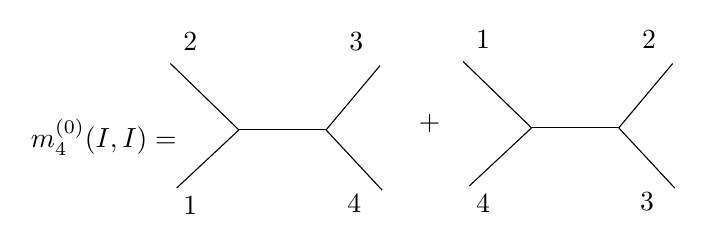
\begin{tikzpicture}[x=0.75pt,y=0.75pt,yscale=-1,xscale=1]
    %uncomment if require: \path (0,300); %set diagram left start at 0, and has height of 300
    
    %Straight Lines [id:da8455657796938298] 
    \draw    (179.5,110) -- (212.5,142) ;
    %Straight Lines [id:da5324594211620186] 
    \draw    (212.5,142) -- (182.5,170) ;
    %Straight Lines [id:da4643902351443361] 
    \draw    (212.5,142) -- (254.5,142) ;
    %Straight Lines [id:da8904360433186445] 
    \draw    (280.5,111) -- (254.5,142) ;
    %Straight Lines [id:da18000644921445508] 
    \draw    (254.5,142) -- (281.5,171) ;
    %Straight Lines [id:da29602344087941934] 
    \draw    (320.5,109) -- (353.5,141) ;
    %Straight Lines [id:da9975053882839713] 
    \draw    (353.5,141) -- (323.5,169) ;
    %Straight Lines [id:da5157442319090852] 
    \draw    (353.5,141) -- (395.5,141) ;
    %Straight Lines [id:da049884375007126946] 
    \draw    (421.5,110) -- (395.5,141) ;
    %Straight Lines [id:da9299487354359295] 
    \draw    (395.5,141) -- (422.5,170) ;
    
    % Text Node
    \draw (111,135.4) node [anchor=north west][inner sep=0.75pt]    {$m_{4}^{(0)}(I,I) =$};
    % Text Node
    \draw (184.5,173) node [anchor=north west][inner sep=0.75pt]   [align=left] {1};
    % Text Node
    \draw (184.5,94) node [anchor=north west][inner sep=0.75pt]   [align=left] {2};
    % Text Node
    \draw (264.5,94) node [anchor=north west][inner sep=0.75pt]   [align=left] {3};
    % Text Node
    \draw (263.5,172) node [anchor=north west][inner sep=0.75pt]   [align=left] {4};
    % Text Node
    \draw (298,133.4) node [anchor=north west][inner sep=0.75pt]    {$+$};
    % Text Node
    \draw (325.5,172) node [anchor=north west][inner sep=0.75pt]   [align=left] {4};
    % Text Node
    \draw (325.5,93) node [anchor=north west][inner sep=0.75pt]   [align=left] {1};
    % Text Node
    \draw (405.5,93) node [anchor=north west][inner sep=0.75pt]   [align=left] {2};
    % Text Node
    \draw (404.5,171) node [anchor=north west][inner sep=0.75pt]   [align=left] {3};
    
    
    \end{tikzpicture}

\end{frame}
\begin{frame}
    Similarly,
    


    \tikzset{every picture/.style={line width=0.75pt}} %set default line width to 0.75pt        

    \begin{tikzpicture}[x=0.75pt,y=0.75pt,yscale=-1,xscale=1]
    %uncomment if require: \path (0,350); %set diagram left start at 0, and has height of 350
    
    %Straight Lines [id:da8963901965951664] 
    \draw    (84,71) -- (108,93) ;
    %Straight Lines [id:da07470927432540231] 
    \draw    (108,93) -- (136,93) ;
    %Straight Lines [id:da12245379377221366] 
    \draw    (108,93) -- (85,111) ;
    %Straight Lines [id:da6511432990080723] 
    \draw    (136,93) -- (161,114) ;
    %Straight Lines [id:da1430135957918477] 
    \draw    (157,71) -- (136,93) ;
    %Straight Lines [id:da8765002291973463] 
    \draw    (157,71) -- (158,47) ;
    %Straight Lines [id:da9623971067643409] 
    \draw    (157,71) -- (178,87) ;
    %Straight Lines [id:da5561877649988292] 
    \draw    (214,70) -- (238,92) ;
    %Straight Lines [id:da44100018812085007] 
    \draw    (238,92) -- (266,92) ;
    %Straight Lines [id:da05824517478761182] 
    \draw    (238,92) -- (215,110) ;
    %Straight Lines [id:da35334338456014613] 
    \draw    (266,92) -- (291,113) ;
    %Straight Lines [id:da9313767826880515] 
    \draw    (287,70) -- (266,92) ;
    %Straight Lines [id:da696534040519218] 
    \draw    (287,70) -- (288,46) ;
    %Straight Lines [id:da5526828548209644] 
    \draw    (287,70) -- (308,86) ;
    %Straight Lines [id:da19124382298581288] 
    \draw    (359,64) -- (383,86) ;
    %Straight Lines [id:da5237814153432139] 
    \draw    (383,86) -- (411,86) ;
    %Straight Lines [id:da7974585866426673] 
    \draw    (383,86) -- (360,104) ;
    %Straight Lines [id:da46316924534551385] 
    \draw    (411,86) -- (436,107) ;
    %Straight Lines [id:da37617479030606993] 
    \draw    (432,64) -- (411,86) ;
    %Straight Lines [id:da9834219129393018] 
    \draw    (432,64) -- (433,40) ;
    %Straight Lines [id:da7117622111604034] 
    \draw    (432,64) -- (453,80) ;
    %Straight Lines [id:da8760088009181417] 
    \draw    (82,171) -- (106,193) ;
    %Straight Lines [id:da7078786925271212] 
    \draw    (106,193) -- (134,193) ;
    %Straight Lines [id:da5389180018159456] 
    \draw    (106,193) -- (83,211) ;
    %Straight Lines [id:da26578622720899636] 
    \draw    (134,193) -- (159,214) ;
    %Straight Lines [id:da5989066756692625] 
    \draw    (155,171) -- (134,193) ;
    %Straight Lines [id:da13747441694892726] 
    \draw    (155,171) -- (156,147) ;
    %Straight Lines [id:da4119117050779677] 
    \draw    (155,171) -- (176,187) ;
    %Straight Lines [id:da5379584617019675] 
    \draw    (221,169) -- (245,191) ;
    %Straight Lines [id:da788296500370655] 
    \draw    (245,191) -- (273,191) ;
    %Straight Lines [id:da4136462405421193] 
    \draw    (245,191) -- (222,209) ;
    %Straight Lines [id:da37414431568833373] 
    \draw    (273,191) -- (298,212) ;
    %Straight Lines [id:da8232480161298765] 
    \draw    (294,169) -- (273,191) ;
    %Straight Lines [id:da7983669347123197] 
    \draw    (294,169) -- (295,145) ;
    %Straight Lines [id:da7903324165137171] 
    \draw    (294,169) -- (315,185) ;
    
    % Text Node
    \draw (5,76.4) node [anchor=north west][inner sep=0.75pt]    {$m_{5}( I,I) =$};
    % Text Node
    \draw (87,114) node [anchor=north west][inner sep=0.75pt]   [align=left] {1};
    % Text Node
    \draw (86,68) node [anchor=south west] [inner sep=0.75pt]   [align=left] {2};
    % Text Node
    \draw (159.5,56) node [anchor=south west] [inner sep=0.75pt]   [align=left] {3};
    % Text Node
    \draw (180,84) node [anchor=south west] [inner sep=0.75pt]   [align=left] {4};
    % Text Node
    \draw (163,111) node [anchor=south west] [inner sep=0.75pt]   [align=left] {5};
    % Text Node
    \draw (198,73.4) node [anchor=north west][inner sep=0.75pt]    {$+$};
    % Text Node
    \draw (217,113) node [anchor=north west][inner sep=0.75pt]   [align=left] {2};
    % Text Node
    \draw (216,67) node [anchor=south west] [inner sep=0.75pt]   [align=left] {3};
    % Text Node
    \draw (289.5,55) node [anchor=south west] [inner sep=0.75pt]   [align=left] {4};
    % Text Node
    \draw (310,83) node [anchor=south west] [inner sep=0.75pt]   [align=left] {5};
    % Text Node
    \draw (293,110) node [anchor=south west] [inner sep=0.75pt]   [align=left] {1};
    % Text Node
    \draw (335,72.4) node [anchor=north west][inner sep=0.75pt]    {$+$};
    % Text Node
    \draw (362,107) node [anchor=north west][inner sep=0.75pt]   [align=left] {3};
    % Text Node
    \draw (361,61) node [anchor=south west] [inner sep=0.75pt]   [align=left] {4};
    % Text Node
    \draw (434.5,49) node [anchor=south west] [inner sep=0.75pt]   [align=left] {5};
    % Text Node
    \draw (455,77) node [anchor=south west] [inner sep=0.75pt]   [align=left] {1};
    % Text Node
    \draw (438,104) node [anchor=south west] [inner sep=0.75pt]   [align=left] {2};
    % Text Node
    \draw (65,184.4) node [anchor=north west][inner sep=0.75pt]    {$+$};
    % Text Node
    \draw (85,214) node [anchor=north west][inner sep=0.75pt]   [align=left] {4};
    % Text Node
    \draw (84,168) node [anchor=south west] [inner sep=0.75pt]   [align=left] {5};
    % Text Node
    \draw (157.5,156) node [anchor=south west] [inner sep=0.75pt]   [align=left] {1};
    % Text Node
    \draw (178,184) node [anchor=south west] [inner sep=0.75pt]   [align=left] {2};
    % Text Node
    \draw (161,211) node [anchor=south west] [inner sep=0.75pt]   [align=left] {3};
    % Text Node
    \draw (201,181.4) node [anchor=north west][inner sep=0.75pt]    {$+$};
    % Text Node
    \draw (224,212) node [anchor=north west][inner sep=0.75pt]   [align=left] {5};
    % Text Node
    \draw (226,172) node [anchor=south west] [inner sep=0.75pt]   [align=left] {1};
    % Text Node
    \draw (296.5,154) node [anchor=south west] [inner sep=0.75pt]   [align=left] {2};
    % Text Node
    \draw (317,182) node [anchor=south west] [inner sep=0.75pt]   [align=left] {3};
    % Text Node
    \draw (300,209) node [anchor=south west] [inner sep=0.75pt]   [align=left] {4};
    
    
    \end{tikzpicture}
\end{frame}
\begin{frame}
    \frametitle{Trivalent graph expansion}
    \begin{alertblock}{Proposition}
        The function $m_n^{(0)}(\alpha|\beta)$ computes the sum of all trivalent scalar diagrams which can be regarded as both $\alpha$ color-ordered and $\beta$ color-orded.
    \end{alertblock}
    \pause
    More explicitly, 
    \begin{equation*}
        \boxed{m_n^{(0)}(\alpha|\beta)=(-1)^{n-3+n_{\text{flip}}(\alpha|\beta)}\sum_{g\in\mathcal{T}(\alpha)\cap\mathcal{T}(\beta)}\prod_{e\in E(g)}\frac{1}{s_e}}
\end{equation*}
where the $\text{flip}(\alpha|\beta)$ is defined below, $\mathcal{T}(\alpha)$ and $\mathcal{T}(\beta)$ refer to the set of color-ordered diagrams in $\alpha$ and 
$\beta$ ordering respectively. To make this expression more clear, see the following diagram
\begin{figure}[htb]
    \centering
    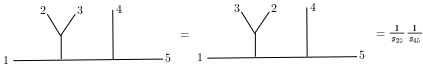
\includegraphics[width=0.8\linewidth]{5.png}
\end{figure}
\end{frame}
\begin{frame}
    We take $m_8^{(0)}(I|18543762)$ as an example to explain how to compute it in an systematic way
    
    %\begin{itemize}
    %    \item First step, draw a disk with n nodes sitting on the boundary in the ordering $\alpha$, then link the n nodes with a loop of line segments according to
    %          the ording $\beta$. The line segments from $\beta$ split the disk into some polygons, like the graph (b). We need to move the external points of every polygon
    %          to make them have no common edges, like graph (c).
    %    \item Second step, put a point in every polygon, named equivalant vertex, and connect this point to all external points in corresponding area. Lines that connect equivalent 
    %          vertices in two regions with common vertices are called equivalent propagators. The resulting graph is an equivalent Feynman diagram, as shown in Figure (d).
    %\end{itemize}
    \begin{figure}
        \centering
        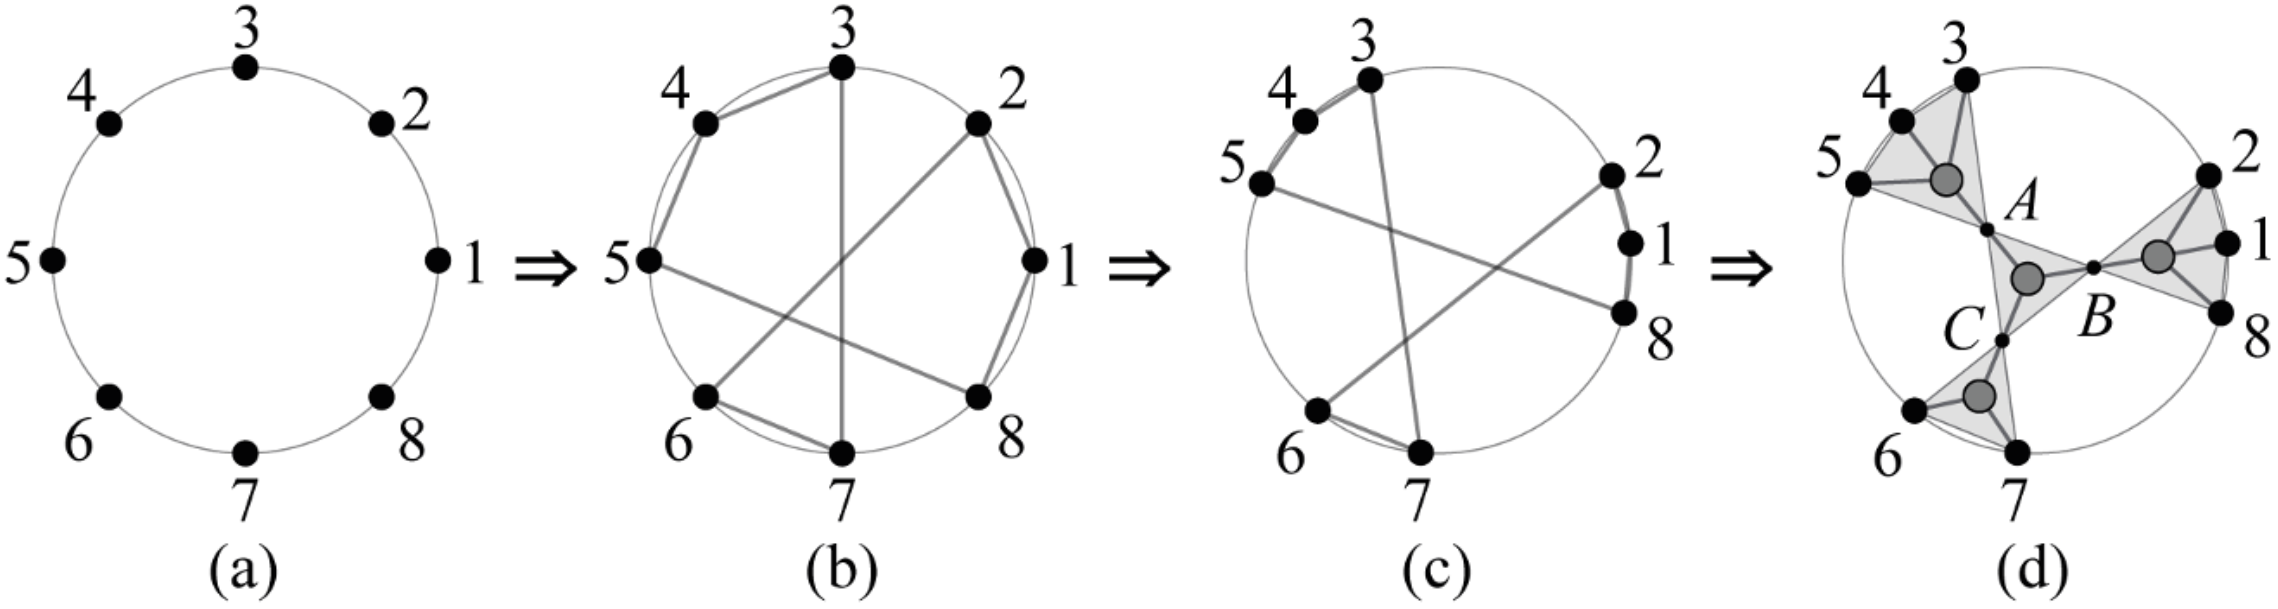
\includegraphics[width=1\linewidth]{7.png}
    \end{figure}
    In this example, we can obtain 
    \begin{equation*}
        m_8^{(0)}(I|54376218)=(-1)^?\left(\frac{1}{s_{21}}+\frac{1}{s_{18}}\right)\left(\frac{1}{s_{34}}+\frac{1}{s_{45}}\right)\frac{1}{s_{345}s_{812}s_{67}}
    \end{equation*}
    As for the indefinite sign, there is also a procedure to determine it.
    
\end{frame}
    
\begin{frame}
    
    %\begin{itemize}
    %    \item Third step, we can read off the corresponding amplitudes from the equivalent Feynman diagram. 
    %\end{itemize}
    %\begin{itemize}
    %\item First step, determine the orientation of the disk by ordering $\alpha$, and define the loop segments by ordering $\beta$, which also determine the orientation of every polygon.
    %    \item Second step, (1) each polygon with odd number vertices contributes a plus sign if the orientation is the same as disk, and a minus sign oppositely;
    %          (2) each polygon with even number vertices contribute a minus sign; (3) each intersection point contributes a minus sign.
    %\end{itemize}
    \begin{figure}
        \centering
        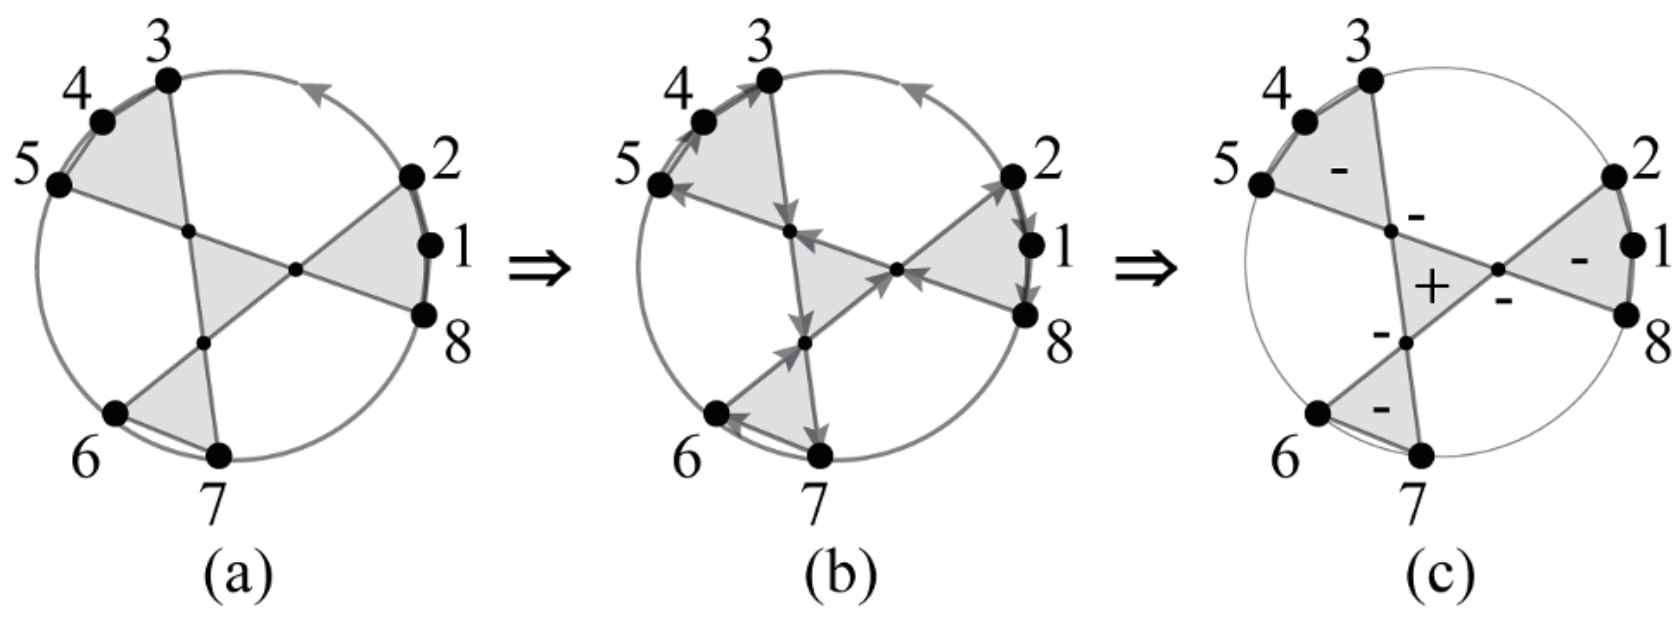
\includegraphics[width=1\linewidth]{6.png}
    \end{figure}
    The final answer is that
    \begin{equation*}
        m_8^{(0)}(I|54376218)=(-1)^6\left(\frac{1}{s_{21}}+\frac{1}{s_{18}}\right)\left(\frac{1}{s_{34}}+\frac{1}{s_{45}}\right)\frac{1}{s_{345}s_{812}s_{67}}
    \end{equation*}
\end{frame}
\begin{frame}
    Now we can unify the color factor and kinematic factor as e in all three theories, so the full amplitude can be written in a unified form
    \begin{equation*}
       \mathcal{M}_n^{(s)}=\sum_{\alpha,\beta\in S_{n-2}}e_\alpha \tilde{e}_\beta m^{(0)}(\alpha|\beta)
    \end{equation*}
    and from the construcion of three type amplitudes, we can obtain
    \begin{equation*}
        {\cal M}^{(0)}_n\times{\cal M}^{(2)}_n={{\cal M}^{(1)}_n}^2
    \end{equation*}
    tree-level BCJ double copy relation.

\end{frame}
\section{Summary and Outlook}
\begin{frame}
    \frametitle{Summary}
    \begin{itemize}
        \item A compact form of tree-level S-matrix in 3 different theories are introduced
            \begin{equation*}
                \mathcal{M}_n^{(s)}=\sum_{\alpha,\beta\in S_{n-2}}e_\alpha e_\beta m^{(0)}(\alpha|\beta)
             \end{equation*}
        \item The computaion method for double partial amplitudes are given 
            \begin{equation*}
                    m_n^{(0)}(\alpha|\beta)=(-1)^{n-3+n_{\text{flip}}(\alpha|\beta)}\sum_{g\in\mathcal{T}(\alpha)\cap\mathcal{T}(\beta)}\prod_{e\in E(g)}\frac{1}{s_e}
            \end{equation*}
        \item The CK duality and BCJ double-copy relation can be easily obtained
            \begin{equation*}
                {\cal M}^{(0)}_n\times{\cal M}^{(2)}_n={{\cal M}^{(1)}_n}^2,\quad e_{g_t}=\pm(e_{g_s}-e_{g_u})
            \end{equation*}
    \end{itemize}
\end{frame}
\begin{frame}
    \frametitle{The most general CHY form}
    In 2013, new formula for tree amplitudes of massless theories has been proposed by Cachazo, He and Yuan:
    \begin{equation*}
        \mathcal{A}=\boxed{\frac{d^n\sigma}{\mathrm{vol\,SL}(2,\mathbb{C})}\prod_a{'}\delta\bigg(\sum_{b\neq a}\frac{s_{ab}}{\sigma_{ab}}\bigg)}\quad \mathcal{I}
    \end{equation*}
    \begin{itemize}
        \item Each particle is represented by a puncture in Riemann sphere.
        \item This form holds for general D-dimension.
        \item The boxed part is \alert{universial for all theories}.
        \item Only the integrand $\mathcal{I}$ determines the particular theory.
    \end{itemize}
\end{frame}
\begin{frame}
    \frametitle{Connection between other theories}
    \begin{figure}
        \centering
        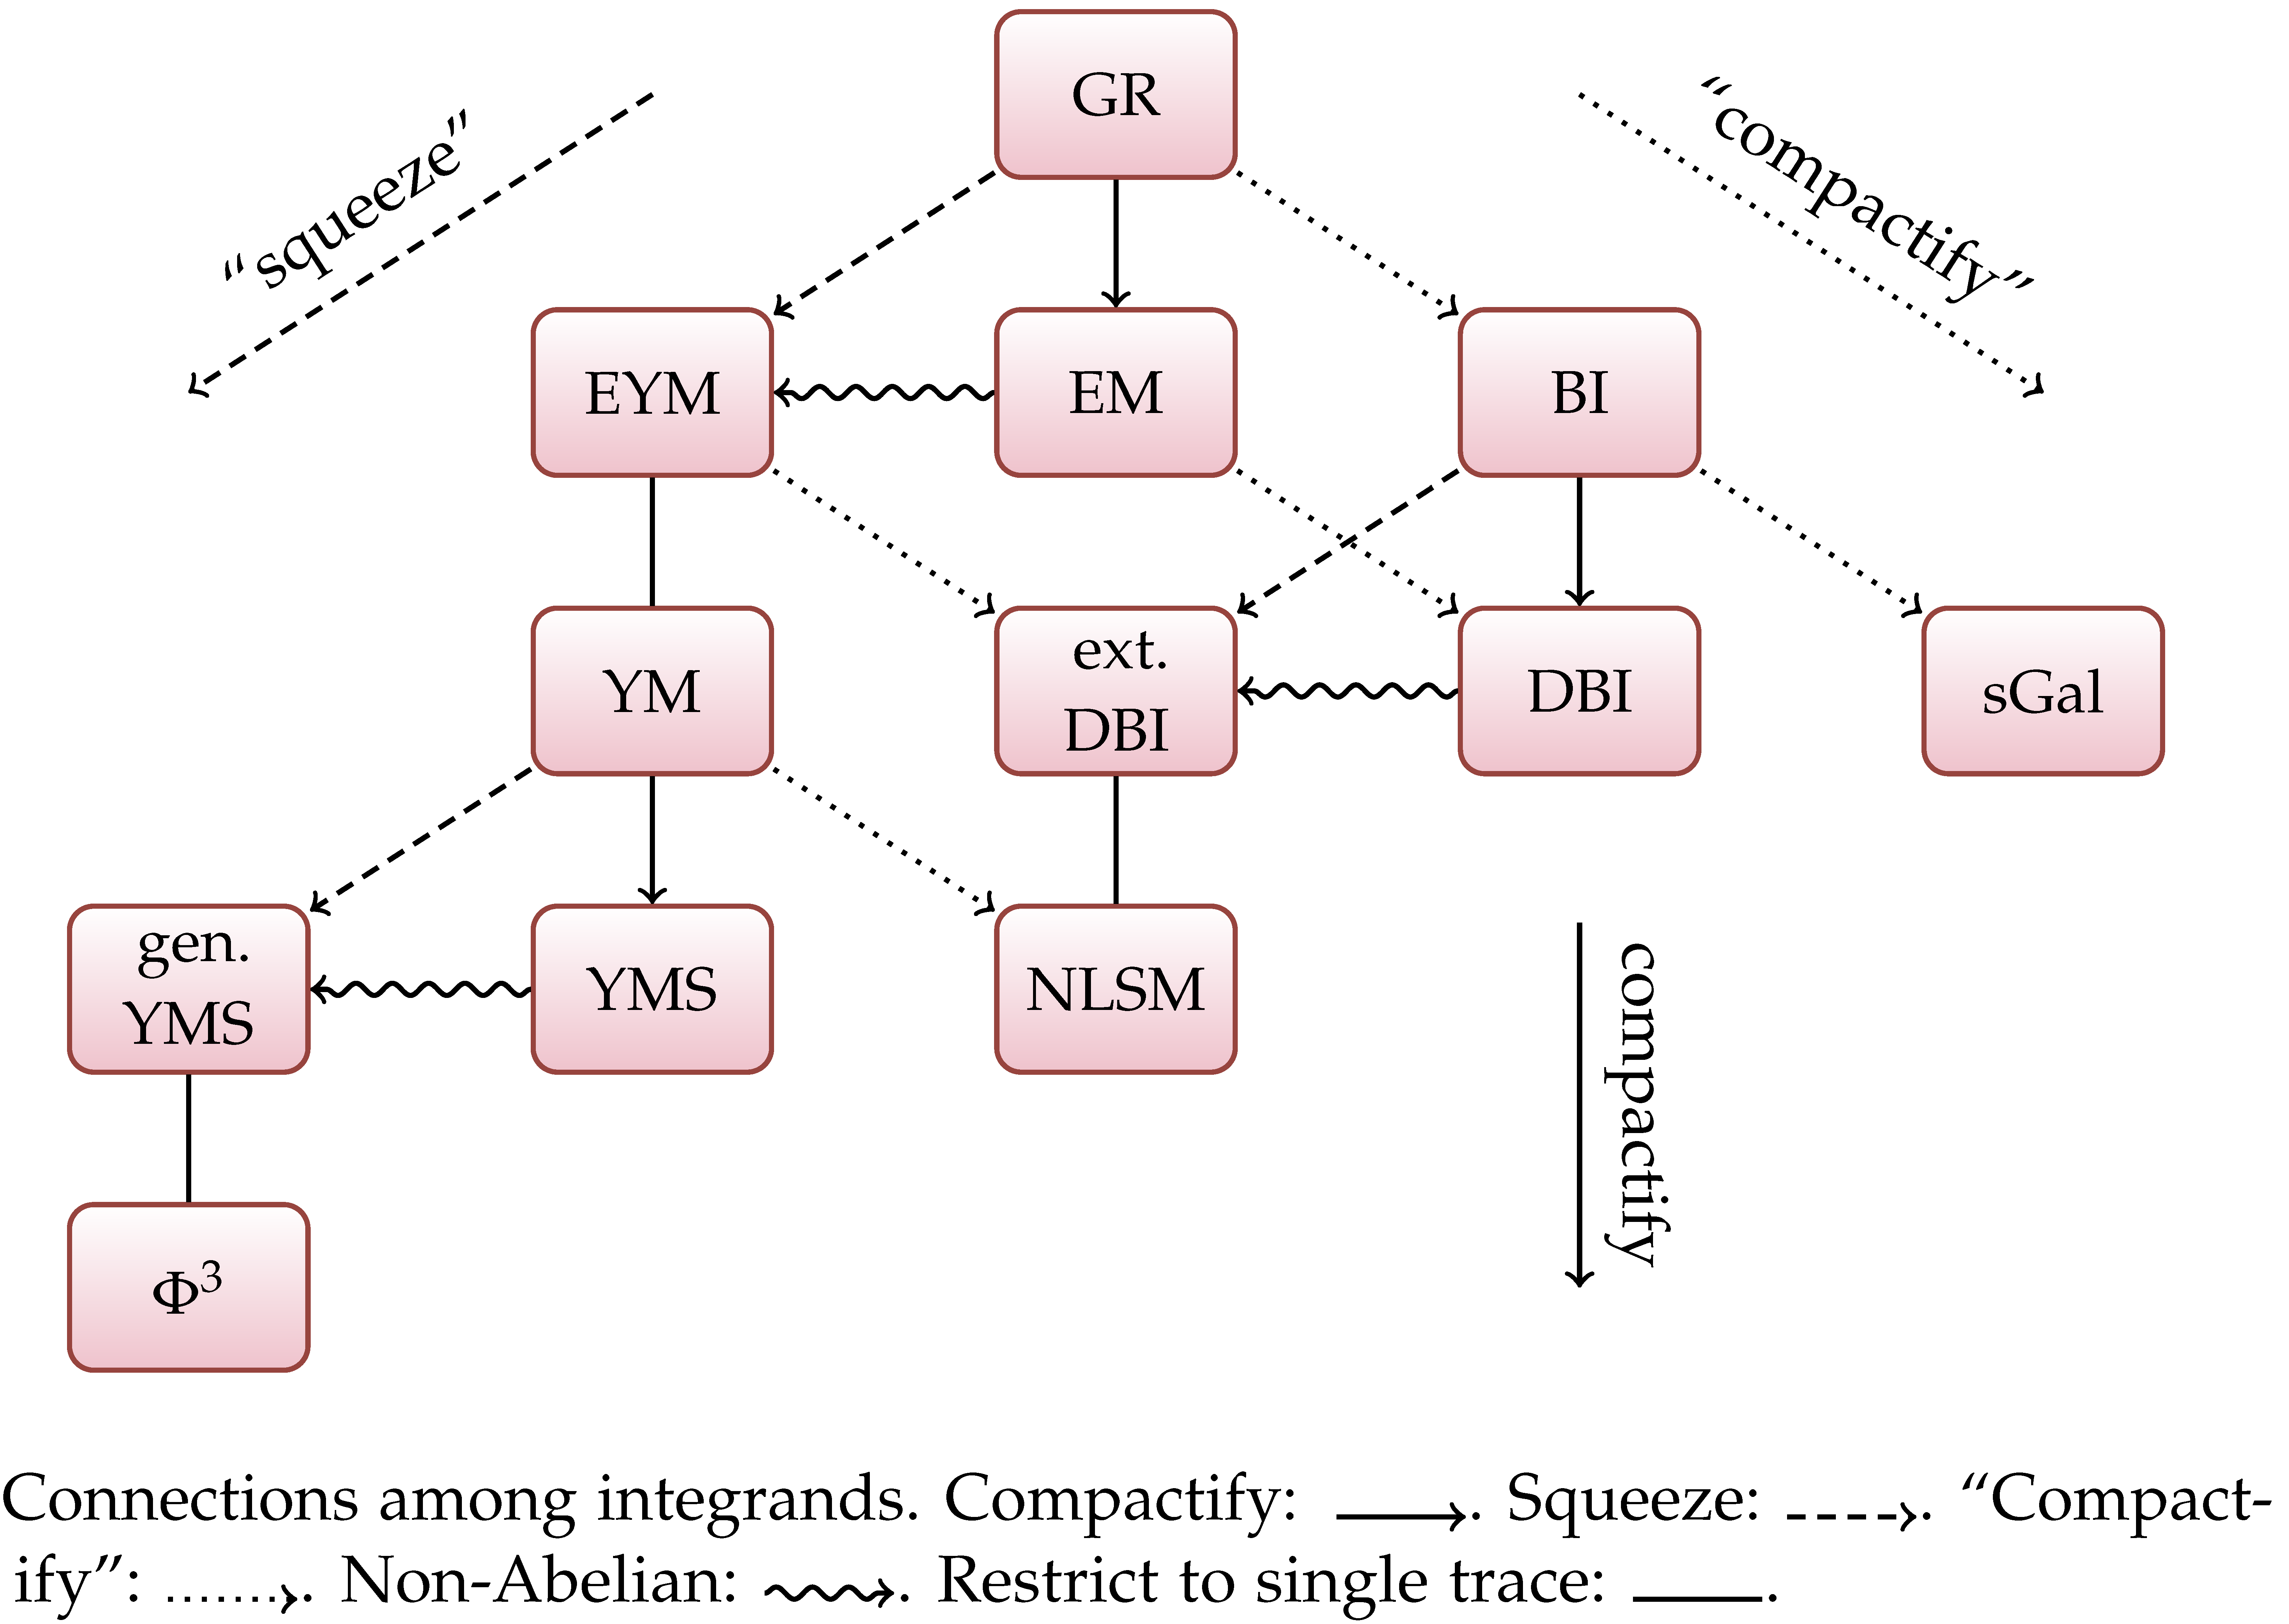
\includegraphics[width=0.8\linewidth]{9.png}
    \end{figure}
\end{frame}
\begin{frame}
    \begin{figure}[t]
        \centering
        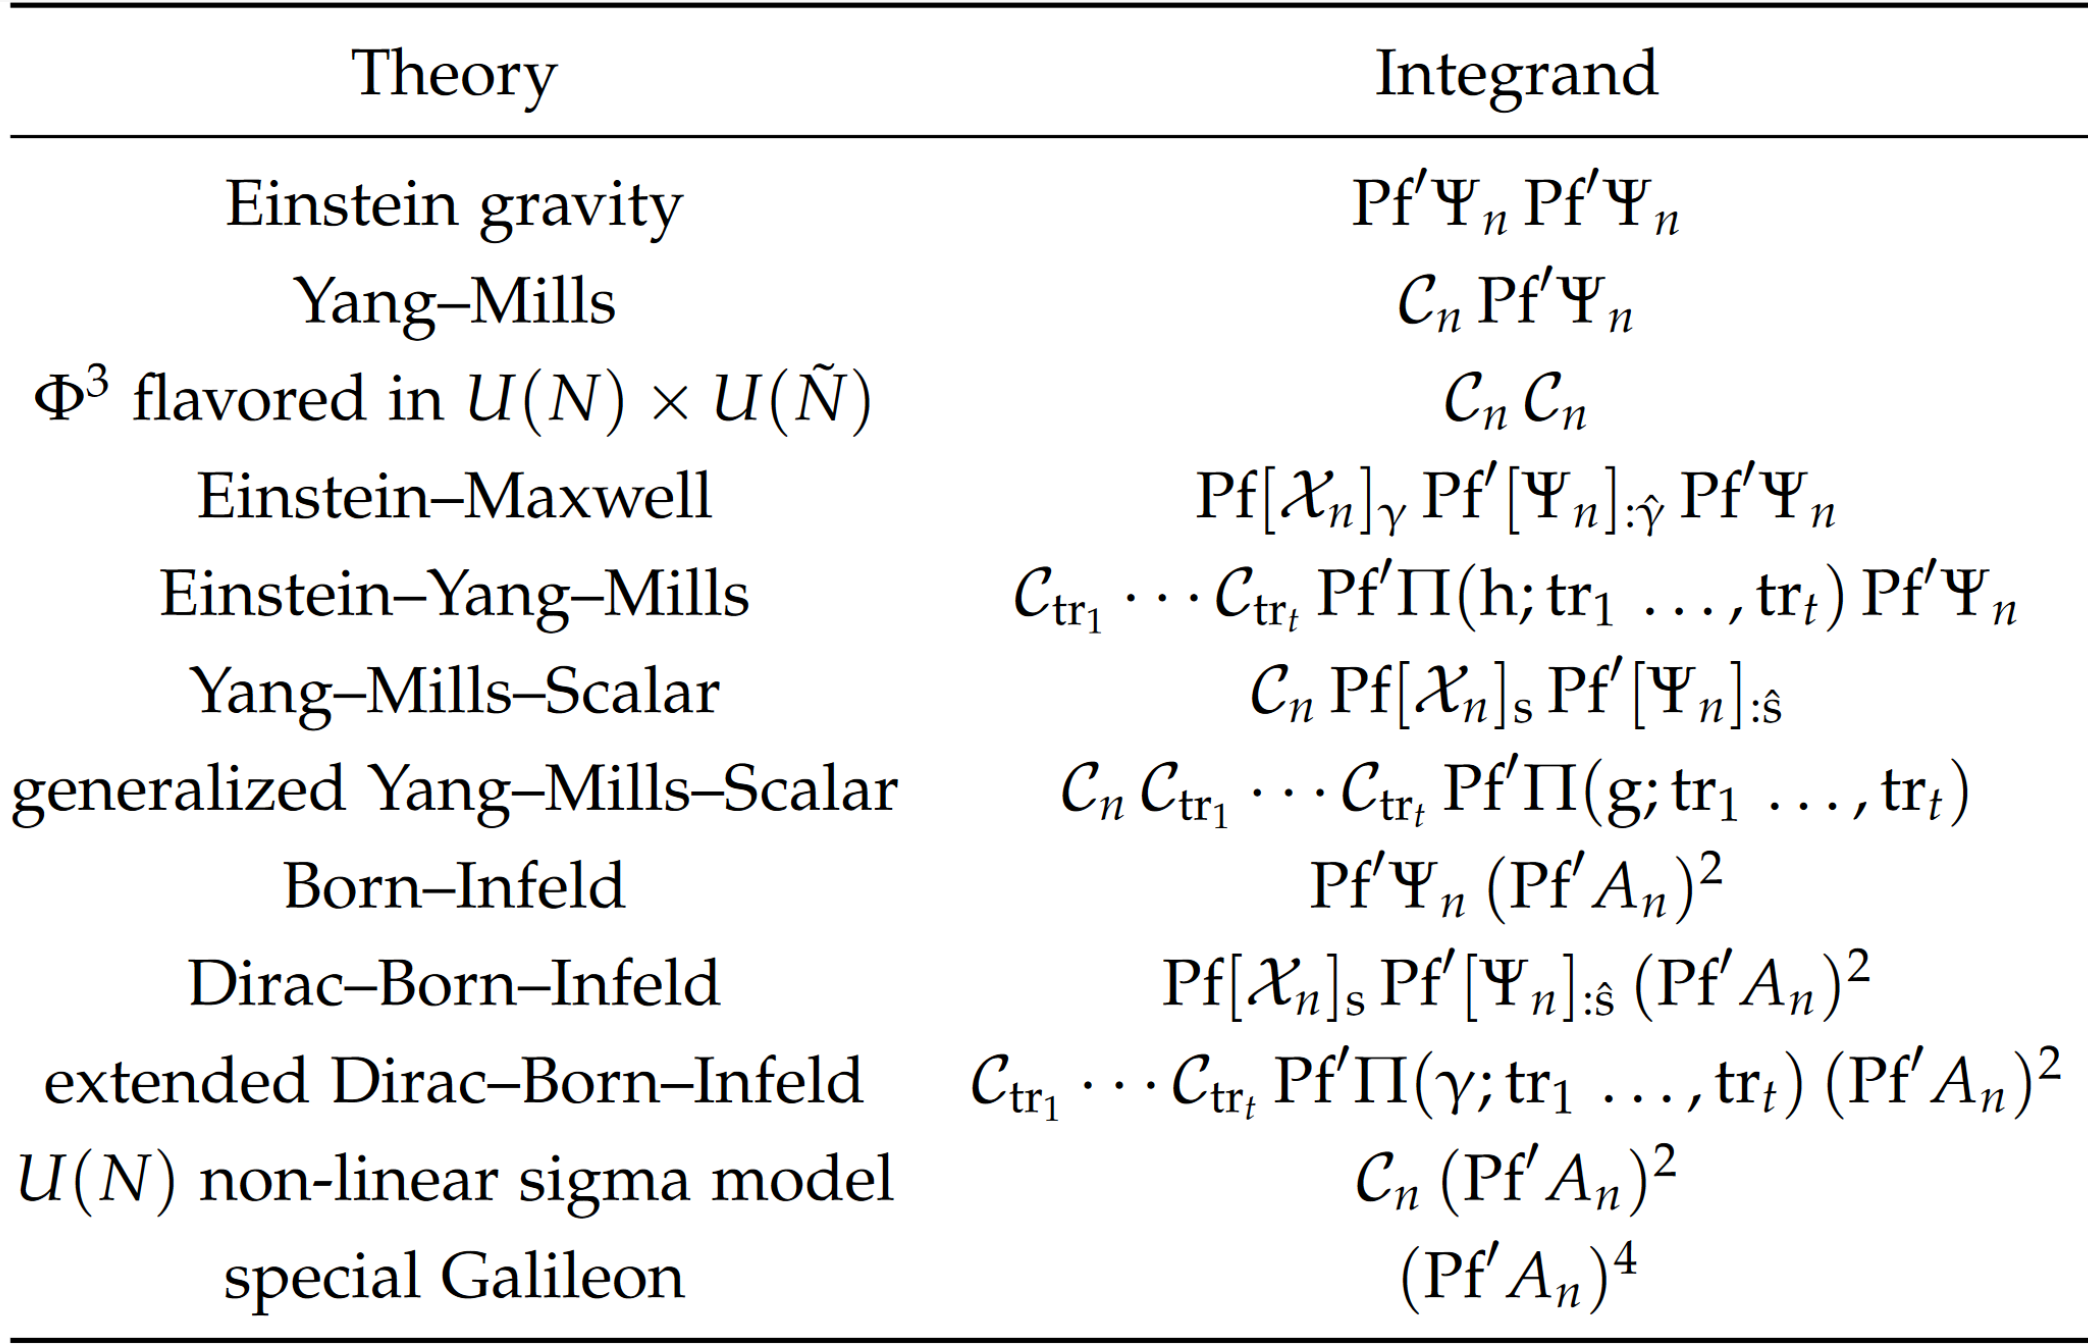
\includegraphics[width=1\linewidth]{4.png}
    \end{figure}
    \alert{arxiv: 1412.3479}
\end{frame}
\begin{frame}
    \centering
    \Huge Thanks for your attention!
\end{frame}
\appendix
\section{Appendix}

\begin{frame}
    The reason we need to write down the measure as this form is that under $\mathrm{SL}(2,\mathbb{C})$
    \begin{align*}
        \sigma_a\to\frac{\alpha\sigma_a+\beta}{\gamma\sigma_a+\delta}:\quad&\prod_{a}{}^{\prime}\delta{\left(\sum_{b\neq a}\frac{s_{ab}}{\sigma_{ab}}\right)}\rightarrow\prod_{a}(\gamma\sigma_a+\delta)^{-2}\prod_{a}{}^{\prime}\delta{\left(\sum_{b\neq a}\frac{s_{ab}}{\sigma_{ab}}\right)}\\
        \quad &d\mu_n\to\prod_{a=1}^n(\gamma\sigma_a+\delta)^{-4}d\mu_n
    \end{align*}
    $E_n(\{k,\epsilon,\sigma\})$ itself is permutaion invariant with resprct to $\sigma_a,k_a^\mu$ and $\epsilon_a^\mu$. The $SL(2,\mathbb{C})$ invariance of amplitude also 
    constraints the form of $E_n(\{k,\epsilon,\sigma\})$
    \begin{equation*}
        \sigma_a\to\frac{\alpha\sigma_a+\beta}{\gamma\sigma_a+\delta}:\quad E_n(\{k,\epsilon,\sigma\})\to E_n(\{k,\epsilon,\sigma\})\prod_{a=1}^n(\gamma\sigma_a+\delta)^2
    \end{equation*}
\end{frame}
\begin{frame}{Gauge theory color structure}
    At tree level, with particles in the adjoint representaion of gauge group SU(N), the amplitude can be 
decomposed as
\textcolor{red}{\begin{equation*}
    \mathcal{A}_n^{tree}(1,2,3,\dots,n)=\sum _{\mathcal{P}(2,3,\dots,n)}Tr[T^{a_1}T^{a_2}T^{a_3}\dots
    T^{a_n}]A_n^{tree}[1,2,3,\dots,n]
\end{equation*}}

here we ommit the coupling constant g, and $A_n^{tree}$ is called tree-level color-ordered partial amplitude.
Notice that this basis includes \textcolor{red}{$(n-1)!$} independent amplitudes.
\end{frame}
\begin{frame}
    Color-ordered partial amplitudes satisfy a set of well-known properties,
    \begin{itemize}
        \item Cyclic:\quad $$A_n^{tree}[1,2,3,\dots,n]=A_n^{tree}[2,3,\dots,n,1]$$
        \item Reflection: \quad $$A_n^{tree}[1,2,3,\dots,n]=(-1)^nA_n^{tree}[n,\dots,3,2,1]$$
        \item "photon" decoupling: \quad $$\sum_{\sigma\in \text{cyclic}}A_n^{tree}[1,\sigma(2,3,\dots,n)]=0$$
        \item KK(Kleiss-Kuijf) relation:\quad $$A_n^{tree}[1,{\alpha},n,{\beta}]=(-1)^{n_\beta}
        \sum_{\left\{\sigma\right\}_i\in OP(\left\{\alpha\right\},\left\{\beta\right\}^T)}A_n^{tree}[1,\left\{\sigma\right\}_i,n]$$
    \end{itemize}
    where the OP means ordered permutaions, that is all permutations of $\left\{\alpha\right\}$$\bigcup$$\left\{\beta\right\}^T$
    that matains the order of individual elements of each set.
\end{frame}
\begin{frame}
    For example, a five point amplitude $A_n^{tree}(1,\{2,3\},5,\{4\})$, we have
\begin{equation*}
    A_n^{tree}[1,2,3,5,4]=-A_n^{tree}[1,2,3,4,5]-A_n^{tree}[1,2,4,3,5]-A_n^{tree}[1,4,2,3,5]
\end{equation*}
The other five point relations can be obtained by permuting legs 2,3,4 and using cyclic and reflection properties.
\\ \hspace*{\fill}\\
This means that the six amplitudes $A_n^{tree}(1,\mathcal{P}\{2,3,4 \},5 )$ form a basis of remaining five-point partial amplitudes.
\textcolor{red}{More generally, for multiplicity n, the KK relation can be used to rewrite any color-ordered partial amplitude in terms of only $(n-2)!$
basis partial amplitudes, where two legs are fixed(usually choose 1 and n).}
\end{frame}
\begin{frame}{A Similar Structure}
    It can be proved that tree level amplitudes can also be decomposed like 
\begin{equation*}
    \mathcal{A}_n^\text{tree}=\sum_{\sigma\in S_{n-2}}\tilde{f}^{a_1a_{\sigma_1}b_1}\tilde{f}^{b_1a_{\sigma_2}b_2}\cdots\tilde{f}^{b_{n-3}a_{\sigma_{n-2}}a_n}\tilde{A}_n(1,\sigma_1,\sigma_2,\ldots,\sigma_{n-2},n)
\end{equation*}
The basis is called DDM and more convenient in parctice. It is easy to realize that the number of basis amplitudes is also \textcolor{red}{$(n-2)!$} with fiexed particle labels 1 and n.
\end{frame}
\begin{frame}
    \begin{Large}
        \textcolor{red}{How can we realize the existence of this basis?}
    \end{Large}
\\ \hspace*{\fill}\\
We just need to notice the contribution from ladder diagram
\begin{figure}[htb]
    \centering
    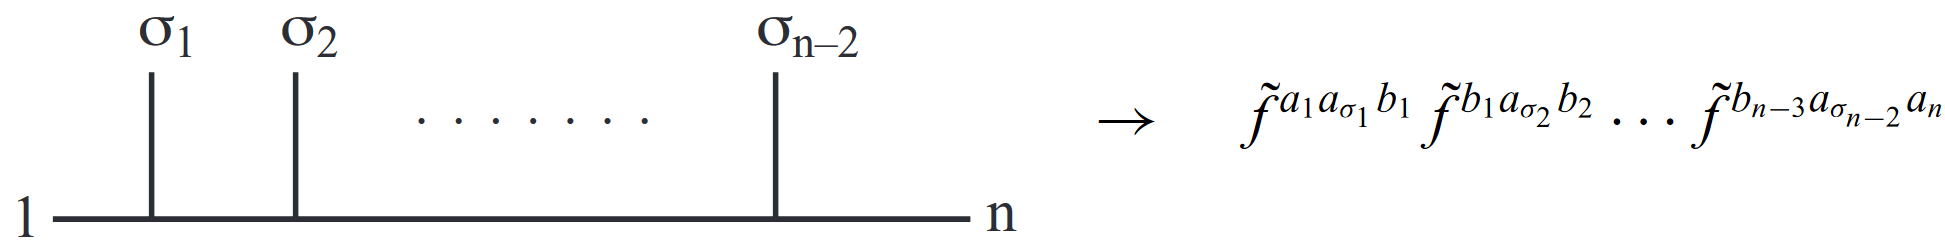
\includegraphics[width=1\linewidth]{1.png}
\end{figure}
And any (three vertex) diagram, by using the Jacobbi identity like 
\begin{figure}[htb]
    \centering
    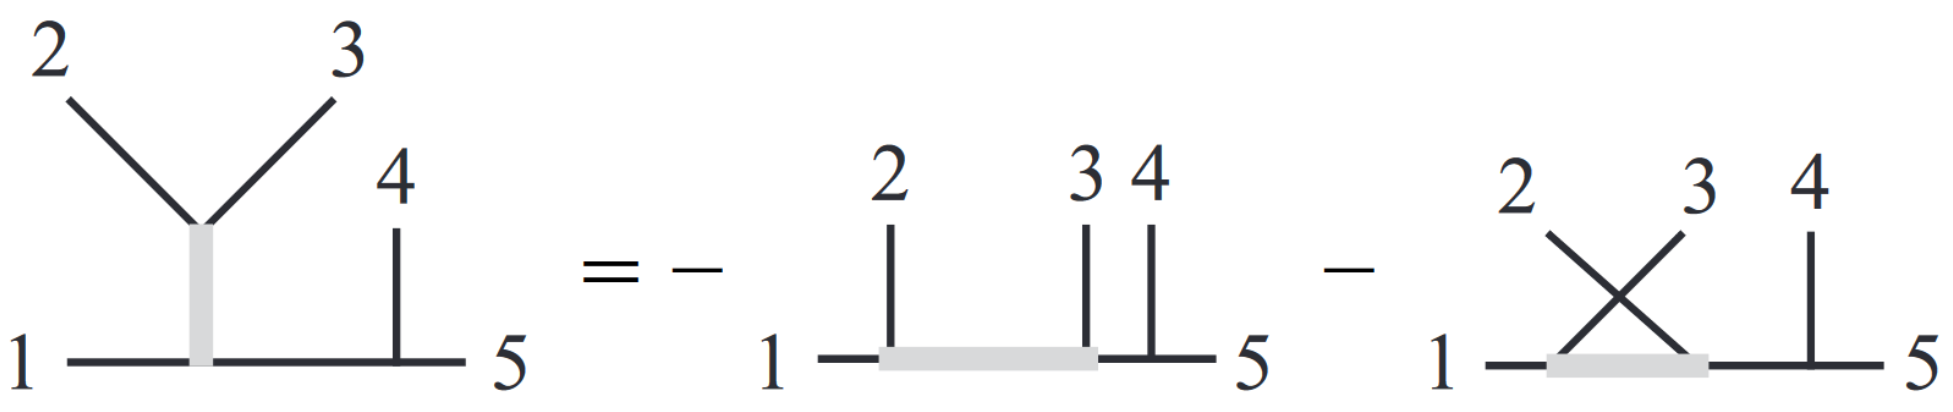
\includegraphics[width=1\linewidth]{2.png}
\end{figure}
can be transformed to the ladder diagram. It has been proved that $\textcolor{red}{\tilde{A}_n(\dots)}$ here is identical to $\textcolor{red}{A_n^{tree}[\dots]}$ in the trace basis.
\end{frame}
\begin{frame}{Color-Kinematics Duality }
The Color-Kinematics Duality here is not the complete version, but we can catch some points.
At four points we have
\begin{equation*}
    A_4^{\mathrm{tree}}(1,2,3,4)+    A_4^{\mathrm{tree}}(1,3,2,4)+    A_4^{\mathrm{tree}}(1,4,2,3)=0.
\end{equation*}
%The decoupling identity does not rely on the specific polariazation and space-time, so the hold of this equation is 
%entirely due to the amplitudes' dependence on Mandelstam variables.
We recognize that the only nontrival way the equation holds accoring to $s+t+u=0$ % Mandelstam variable
\begin{align*}
    &A_4^{\mathrm{tree}}(1,2,3,4)+    A_4^{\mathrm{tree}}(1,3,2,4)+    A_4^{\mathrm{tree}}(1,4,2,3)\\
\quad&= (s+t+u)\chi=0
\end{align*} 
Considering that $A_4^{\mathrm{tree}}(1,2,3,4)$ treats $s$ and $t$ the same, and similar to the other two, we make the identification
\begin{equation*}
    A_4^{\mathrm{tree}}(1,2,3,4)=u\chi,\quad   A_4^{\mathrm{tree}}(1,3,2,4)=t\chi,\quad    A_4^{\mathrm{tree}}(1,4,2,3)=s\chi
\end{equation*}
\end{frame}
\begin{frame}
    We obtain
    \begin{align*}
        tA_4^{\mathrm{tree}}(1,2,3,4)=uA_4^{\mathrm{tree}}(1,3,4,2),\\
        sA_4^{\mathrm{tree}}(1,2,3,4)=uA_4^{\mathrm{tree}}(1,4,2,3),\\
        tA_4^{\mathrm{tree}}(1,2,3,4)=sA_4^{\mathrm{tree}}(1,3,4,2).\\
    \end{align*}
    And in order to obtain the knematic analog of Jacobbi identity, it is convenient to express the amplitudes in terms of poles
\begin{align*}
    &A_4^{\mathrm{tree}}(1,2,3,4)\equiv\frac{n_s}{s}+\frac{n_t}{t},\\
    &A_4^{\mathrm{tree}}(1,3,4,2)\equiv-\frac{n_u}{u}-\frac{n_s}{s},\\
    &A_4^{\mathrm{tree}}(1,4,2,3)\equiv-\frac{n_t}{t}+\frac{n_u}{u}.
\end{align*}
the relative sign here is just a convention.
\end{frame}
\begin{frame}
    Combining the two relation above gives the desired identity
    \begin{equation*}
        \alert{n_u=n_s-n_t}
    \end{equation*}
    this is exactly the same form of Jacobbi identity for the color factors.
    The full amplitude can be written like
\begin{equation*}
    \mathcal{A}_4^{\mathrm{tree}}=g^2\left(\frac{n_sc_s}{s}+\frac{n_uc_u}{u}+\frac{n_tc_t}{t}\right)
\end{equation*}
\end{frame}
\begin{frame}
    For the five point case, an example is 
    \begin{figure}[htb]
        \centering
        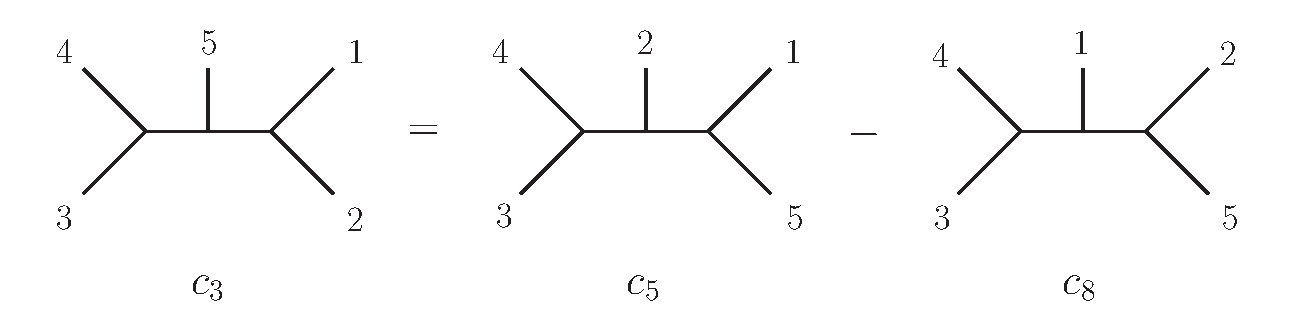
\includegraphics[width=1\linewidth]{FivePtTwist2.eps}
    \end{figure}
    we have the corresponding color factor Jacobbi identities like
    \begin{equation*}
        c_3=c_5-c_8
    \end{equation*}
    so we need to have the knematic analog
    \begin{equation*}
        n_3=n_5-n_8
    \end{equation*}
    The explict forms of all these factors can be found in the original paper \textbf{New relations for gauge theory amplituds, PRD 78, 085011}
\end{frame}
\begin{frame}
    Full amplitudes of 5 points are
    \begin{eqnarray*}
        \mathcal {A}^\mathrm{tree}_5& = & 
        g^3\Biggl( {n_1 c_1\over s_{12}s_{45}}+{n_2 c_2\over s_{23}s_{51}}
        +{n_3 c_3 \over s_{34}s_{12}}+{n_4 c_4\over s_{45}s_{23}}
        +{n_5 c_5\over s_{51}s_{34}} +{n_{6} c_6\over s_{14}s_{25}}  \\
        &&\null \hskip .3 cm 
        + {n_7 c_7\over s_{32}s_{14}}+{n_{8} c_8\over s_{25}s_{43}}
        +{n_{9} c_9\over s_{13}s_{25}}+{n_{10} c_{10}\over s_{42}s_{13}}
        +{n_{11} c_{11}\over s_{51}s_{42}}+ {n_{12} c_{12}\over s_{12}s_{35}}  \\
        &&\null \hskip .3 cm 
        +{n_{13} c_{13}\over s_{35}s_{24}} 
        +{n_{14} c_{14}\over s_{14}s_{35}}
        +{n_{15} c_{15}\over s_{13}s_{45}}\Biggr)\,,
        \end{eqnarray*}
    This relation had been proved upto 8 points at the time and I think it has been improved to arbitrary points.  
\end{frame}
\begin{frame}{KLT Relation}
    So-called KLT relation, in the language of field theory, refers to the decomposition of \alert{gravity amplitudes} to \alert{two gauge theory amplitues}. 
    \begin{table}[]
        \resizebox{\textwidth}{!}{
        \begin{tabular}{|l|l|l|l|l|}
        \hline
         \(\mathcal{N}\) & Factors & Supergravity   \\ \hline
         8 &   \(\mathcal{N}=4SYM\otimes \mathcal{N}=4SYM\)      &   pure \(\mathcal{N}=8 \)SG             \\ \hline
         6 &   \(\mathcal{N}=4SYM\otimes \mathcal{N}=2SYM\)      &   pure \(\mathcal{N}=6 \)SG             \\ \hline
         5 &   \(\mathcal{N}=4SYM\otimes \mathcal{N}=1SYM\)      &   pure \(\mathcal{N}=5 \)SG             \\ \hline
         4 &   \(\mathcal{N}=4SYM\otimes (\mathcal{N}=0YM+n_\nu scalars)\)      &    \(\mathcal{N}=4 \)SG,\(n_\nu\)vector multiplets             \\ \hline
         4 &   \(\mathcal{N}=2SYM\otimes \mathcal{N}=2SYM\)      &    \(\mathcal{N}=4 \)SG,2 vector multiplets            \\ \hline
         3 &   \(\mathcal{N}=2SYM\otimes \mathcal{N}=1SYM\)      &    \(\mathcal{N}=3 \)SG,1 vector multiplet           \\ \hline
         2 &   \(\mathcal{N}=2SYM\otimes (\mathcal{N}=0YM+n_\nu scalars)\)      &    \(\mathcal{N}=2 \)SG,\(n_\nu\) multiplets+1 vector multiplets            \\ \hline
         2 &   \(\mathcal{N}=1SYM\otimes \mathcal{N}=1SYM\)       &    \(\mathcal{N}=2 \)SG ,1 hypermultiplet               \\ \hline
         1 &   \(\mathcal{N}=1SYM\otimes (\mathcal{N}=0YM+n_\nu scalars)\)      &     \(\mathcal{N}=1 \)SG,  \(n_\nu\) vector and 1 chiral multiplet           \\ \hline
        \end{tabular}
        }
        \end{table}
\end{frame}


\begin{frame}{KLT Orthogonality}
    $\bullet$ KLT orthogonality is a striking property of the solutions to scattering equations.
    \begin{block}{Proposition 1}
        \begin{equation*}
            \frac{(i,j)}{(i,i)^{\frac12}(j,j)^{\frac12}}=\delta_{ij}
        \end{equation*}
    \end{block}
    
\end{frame}
\begin{frame}
    First we need to define the Jacobian matrix associated to the scattering equations
        
        \begin{equation*}
            \boxed{
            \label{jacobbi}
            \Phi_{ab}\equiv\partial\left(\sum_{c\neq a}\frac{s_{ac}}{\sigma_a-\sigma_c}\right)/\left(\partial\sigma_b\right)=\begin{cases}\frac{s_{ab}}{(\sigma_a-\sigma_b)^2},&a\neq b,\\-\sum_{c\neq a}\Phi_{ac}, &a=b\end{cases}
            }
        \end{equation*}
    As mentioned above only n-3 of the scattering equations are independent so the matrix $\Phi$ has \alert{rank n-3}.  (This matrix was first encountered in the gravity amplitudes constructed from gauge theory using KLT relation ) 
\end{frame}
\begin{frame}
    Consider a generalization of $\Phi_{ab}$ 
    \begin{equation*}
        \Psi_{ab,a\neq b}\equiv\frac{s_{ab}}{(\sigma_a-\sigma_b)(\sigma_a^{\prime}-\sigma_b^{\prime})},\quad\Psi_{aa}\equiv-\sum_{c\neq a}\Psi_{ac}.
    \end{equation*}
    \begin{block}{Proposition 2}
        \begin{equation*}
            \operatorname{rank}\Psi(\{\sigma\},\{\sigma^{\prime}\})=\begin{cases}n-4, \{\sigma\}\neq\{\sigma^{\prime}\}\\n-3, \{\sigma\}=\{\sigma^{\prime}\}\end{cases}
        \end{equation*}
        $\sigma$ and $\sigma^\prime$ are assmused to be solutions to scattering equation.
    \end{block}
\end{frame}
\begin{frame}{Prove of KLT orthogonality}
    For the purpose of proving KLT orthogonality, we can construct a n! dimension vector for each solution
    \begin{equation*}
        \frac1{(\sigma_{\omega(1)}-\sigma_{\omega(2)})(\sigma_{\omega(2)}-\sigma_{\omega(3)})\cdots(\sigma_{\omega(n)}-\sigma_{\omega(1)})}
    \end{equation*}
    Not so obvious is the fact that we can fix the positon of 3 labels, which we choose 1,n-1,n, give rise to the KK relation and BCJ relation.
    \\ \hspace*{\fill}\\
    Now the vectors become (n-3)! dimension, and even aftering selecting three lables, we still have the freedom of where to put them. Here we only use two choices :
    \begin{equation*}
        \textcolor{red}{(1,\omega(2),\dots,\omega(n-2),n-1,n)\quad and \quad (1,\omega(2),\dots,\omega(n-2),n,n-1 )}
    \end{equation*}
\end{frame}
\begin{frame}
    The corresponding two vectors are 
    \begin{align*}V(\omega)&=\frac1{(\sigma_1-\sigma_{\omega(2)})\cdots(\sigma_{\omega(n-2)}-\sigma_{n-1})(\sigma_{n-1}-\sigma_n)(\sigma_n-\sigma_1)},\\U(\omega)&=\frac1{(\sigma_1-\sigma_{\omega(2)})\cdots(\sigma_{\omega(n-2)}-\sigma_n)(\sigma_n-\sigma_{n-1})(\sigma_{n-1}-\sigma_1)}.
    \end{align*}
    In this language, we can construct a bilinear form 
    \begin{equation*}
        S[\alpha|\beta]=\prod^{n-2}_{i=2}\left(s_{1,\alpha_i}+\sum_{j=2}^{i-1}
        \theta(\alpha(j),\alpha(i))_\beta s_{\alpha(j),\alpha(i)}\right)
    \end{equation*}
    where $\alpha,\beta\in S_{n-3}$,$\theta(i,j)_\beta=1$if the order of i,j is the same in both permutations 
    $\alpha(2,3,\dots,n-2)$ and $\beta(2,3,\dots,n-2)$, and 0 otherwise.
    S is usually called \alert{Momentum Kernel}.
\end{frame}
\begin{frame}
    Given any two solutions of scatering equations,
    \begin{equation*}
        \{\sigma_1^{(i)},\sigma_2^{(i)},\dots,\sigma_n^{(i)}\}\quad and \quad \{\sigma_1^{(j)},\sigma_2^{(j)},\dots,\sigma_n^{(j)}\}
    \end{equation*}
    define two vectors, $V(\alpha)^{(i)}$ and $U(\beta)^{(j)}$, i,j are choices of solutions and $\alpha,\beta$ are the choices of permutaions,
    the number of both is \alert{(n-3)!}.
    \\ \hspace*{\fill}\\
    A natural inner product can be defined as
    \begin{equation*}
        (i,j):=\sum_{\alpha,\beta\in S_{n-3}}V^{(i)}(\alpha)S[\alpha|\beta]U^{(j)}(\beta)
    \end{equation*}
    Knowing all definetions above, we can proceed to prove KLT orthogonality.
\end{frame}
\begin{frame}
    The starting point is to notice that
    \begin{equation*}
        \frac{(i,j)}{(i,i)^{\frac12}(j,j)^{\frac12}}=\delta_{ij}
    \end{equation*}
    is clearly invariant under $SL(2,\mathbb{C})\times SL(2,\mathbb{C})$. Partially fixing both $SL(2,\mathbb{C})$
    redundancies with convenient choice $\sigma_{n-1}^{(i)}=\sigma_n^{(j)}=\infty$ and $\sigma_n^{(i)}=\sigma_{n-1}^{(j)}=1$
    and define 
    \begin{align*}
            K_n(\{\sigma\},\{\sigma'\})\equiv\sum_{\alpha,\beta\in S_{n-3}}&\frac1{\sigma_{1,\alpha(2)}\ldots\sigma_{\alpha(n-3),\alpha(n-2)}}S[\alpha|\beta]\\
            &\frac1{\sigma_{1,\beta(2)}^{\prime}\ldots\sigma_{\beta(n-3),\beta(n-2)}^{\prime}}
    \end{align*}
    The motivation for this definition is that $K_n$ appears in the numerator of KLT orthogonality.
\end{frame}
\begin{frame}
    It is also convenient to define an auxiliary co-rank one $(n-2)\times(n-2)$ matrix $\psi^{(n)}$
    \begin{equation*}
        \psi_{ab,a\neq b}=\frac{s_{ab}}{\sigma_{ab}\sigma_{ab}^{\prime}},\quad\psi_{aa}=-\sum_{b\neq a}\psi_{ab},\quad a,b=1,\ldots,n{-}2
    \end{equation*}
    It can be proven that any $(n-3)\times(n-3)$ minors of $\psi^{(n)}$ are the same, and we denote such a minor as
    ${\det}^\prime\psi^{(n)}$ , that is to say, the determinat of the matrix after removing any row and colum.
    \begin{block}{Proposition 3}
        The two functions defined above are identical up to a sign.
        \begin{equation*}
            K_n(\{\sigma\},\{\sigma'\})=(-1)^n{\det}^\prime\psi^{(n)}
        \end{equation*}
    \end{block}
\end{frame}
\begin{frame}
    The final step is put all pieces together. With the choice  $\sigma_{n-1}^{(i)}=\sigma_n^{(j)}=\infty$ and $\sigma_n^{(i)}=\sigma_{n-1}^{(j)}=1$,
    we have 
    \begin{equation*}
        \frac{(i,j)}{(i,i)^{\frac12}(j,j)^{\frac12}}=\frac{K_n(\{\sigma^{(i)}\},\{\sigma^{(j)}\})}{K_n^{\frac12}(\{\sigma^{(i)}\},\{\sigma^{(i)}\})K_n^{\frac12}(\{\sigma^{(j)}\},\{\sigma^{(j)}\})}
    \end{equation*}
    In addition, one finds that the minor of $\psi$ obtained by removing the first row and colum is identical to 
    that of $\Psi(\{\sigma\},\{\sigma^{\prime}\})$ after removing rows and colums $\{1,n-1,n\}$. We denote them respectively
    $|\psi^{(n)}|^1_1$ and $|\Psi|^{1,n-1,n}_{1,n-1,n}$. Then,
    \begin{align*}
        \frac{(i,j)}{(i,i)^{\frac12}(j,j)^{\frac12}}&=\frac{K_n(\{\sigma^{(i)}\},\{\sigma^{(j)}\})}{K_n^{\frac12}(\{\sigma^{(i)}\},\{\sigma^{(i)}\})K_n^{\frac12}(\{\sigma^{(j)}\},\{\sigma^{(j)}\})}\\
        &=\frac{(-1)^n|\psi^{(n)}|^1_1}{{(-1)^n|\psi^{(n)}|^1_1}^{\frac{1}{2}}{|\psi^{(n)}|^1_1}^{\frac{1}{2}}}\\
        &=\frac{|\Psi(\{\sigma^{(i)}\},\{\sigma^{(j)}\})|_{1,n-1,n}^{1,n-1,n}}{(|\Psi(\{\sigma^{(i)},\sigma^{(i)}\}|_{1,n-1,n}^{1,n-1,n})^{\frac12}(|\Psi(\{\sigma^{(j)}\},\{\sigma^{(j)}\}|_{1,n-1,n}^{1,n-1,n})^{\frac12}}
    \end{align*}
\end{frame}
\begin{frame}
    Fianlly, we just need to use Proposition 2. 
    \begin{itemize}
        \item If $i=j$, the rank of matrix $\Psi$ is $n-3$ and the minor is nonzero, we obtain
        \begin{equation*}
            \frac{(i,i)}{(i,i)^{\frac12}(i,i)^{\frac12}}=\frac{|\Psi(\{\sigma^{(i)}\},\{\sigma^{(j)}\})|_{1,n-1,n}^{1,n-1,n}}{|\Psi(\{\sigma^{(i)}\},\{\sigma^{(j)}\})|_{1,n-1,n}^{1,n-1,n}}=1
        \end{equation*}
        \item If $i\neq j$, the rank of matrix is $n-4$, so any minor with volume more than $n-4$ equals 0.
        \begin{equation*}
            |\Psi(\{\sigma^{(i)}\},\{\sigma^{(j)}\})|_{1,n-1,n}^{1,n-1,n}=0\Rightarrow \frac{(i,j)}{(i,i)^{\frac12}(j,j)^{\frac12}}=0
        \end{equation*}
    \end{itemize}
    Up to now, we conclude the proof of KLT orthogonality.
\end{frame}
\begin{frame}
    \frametitle{Attempt to construct S-matrix --- Towards CHY}
    Thanks to the excellent properties of scattering equations, it is very tempting to propose that the solutions
    to scattering equations should be used to construct scattering amplitudes.
    \\ \hspace*{\fill}\\
    The first two constructed are YM and gravity amplitudes in any dimensions
    \begin{align*}
        M_n^{\mathrm{YM}}(1,2,\dots,n)&=\int\frac{d^n\sigma}{\text{vol SL}(2,\mathbb{C})}\prod_a{'}\delta\bigg(\sum_{b\neq a}\frac{s_{ab}}{\sigma_{ab}}\bigg)\frac{E_n(\{k,\epsilon,\sigma\})}{\sigma_{12}\dots\sigma_{n1}},\\
        M_n^{\mathrm{gravity}}&=\int\frac{d^n\sigma}{\text{vol SL}(2,\mathbb{C})}\prod_a{'}\delta\bigg(\sum_{b\neq a}\frac{s_{ab}}{\sigma_{ab}}\bigg)E_n(\{k,\epsilon,\sigma\})^2
    \end{align*}
    The measure is defined as following
    \begin{equation*}
        \prod_{a}{}^{\prime}\delta{\left(\sum_{b\neq a}\frac{s_{ab}}{\sigma_{ab}}\right)}{:}=\sigma_{ij}\sigma_{jk}\sigma_{ki}\prod_{a\neq i,j,k}\delta{\left(\sum_{b\neq a}\frac{s_{ab}}{\sigma_{ab}}\right)}
    \end{equation*}
\end{frame}
\begin{frame}
    The reason we extract 3 indices from delta equation is the fact that only $n-3$ scattering equations are independent.
    This from can be proved to be \alert{independent of choice of $i,j,k$}, therefore permutaion invariant.
    We also have
    \begin{equation*}
        \sigma_a\to\frac{\alpha\sigma_a+\beta}{\gamma\sigma_a+\delta}:\quad d\mu_n\to\prod_{a=1}^n(\gamma\sigma_a+\delta)^{-4}d\mu_n
    \end{equation*}
    $E_n(\{k,\epsilon,\sigma\})$ itself is permutaion invariant with resprct to $\sigma_a,k_a^\mu$ and $\epsilon_a^\mu$. The $SL(2,\mathbb{C})$ invariance of amplitude also 
    constraints the form of $E_n(\{k,\epsilon,\sigma\})$
    \begin{equation*}
        \sigma_a\to\frac{\alpha\sigma_a+\beta}{\gamma\sigma_a+\delta}:\quad E_n(\{k,\epsilon,\sigma\})\to E_n(\{k,\epsilon,\sigma\})\prod_{a=1}^n(\gamma\sigma_a+\delta)^2
    \end{equation*}
\end{frame}
\begin{frame}{The form of measure}
    It is worth to computed the measure explicitly.Aftering "gauge fixing" the $SL(2,\mathbb{C})$ redundancy, one finds 
    \begin{equation*}
        \int\prod_{c\neq p,q,r}d\sigma_c(\sigma_{pq}\sigma_{qr}\sigma_{rp})(\sigma_{ij}\sigma_{jk}\sigma_{ki})\prod_{a\neq i,j,k}\delta\biggl(\sum_{b\neq a}\frac{s_{ab}}{\sigma_{ab}}\biggr)
    \end{equation*}
    The delta functions completely localize all integrals and the answer is evaluating a Jacobian defined above.
    \begin{equation*}
            \Phi_{ab}\equiv\partial\left(\sum_{c\neq a}\frac{s_{ac}}{\sigma_a-\sigma_c}\right)/\left(\partial\sigma_b\right)=\begin{cases}\frac{s_{ab}}{(\sigma_a-\sigma_b)^2},&a\neq b,\\-\sum_{c\neq a}\Phi_{ac}, &a=b\end{cases}
    \end{equation*}
    Then, we obtain the measure
    \begin{equation*}
            \boxed{
            \sum_{\{\sigma\}\in\mathrm{solutions}}\frac{(\sigma_{pq}\sigma_{qr}\sigma_{rp})(\sigma_{ij}\sigma_{jk}\sigma_{ki})}{|\Phi|_{pqr}^{ijk}}}
    \end{equation*}
\end{frame}
\begin{frame}
    Always denoted by 
    \begin{equation*}
        \boxed{
        \det{'}\Phi:=\frac{|\Phi|_{pqr}^{ijk}}{(\sigma_{pq}\sigma_{qr}\sigma_{rp})(\sigma_{ij}\sigma_{jk}\sigma_{ki})}}
    \end{equation*}
    $|\Phi|_{pqr}^{ijk}$ means that we need to delete the rows $\{i,j,k\}$ and the colums $\{p,q,r\}$, of course it is free to choose which inedex refers
    to row or colum ($\Phi$ is a symmetric matrix).
\end{frame}
\begin{frame}
    \frametitle{The form of $E_n(\{k,\epsilon,\sigma\})$}
    In order to present the explict form of $E_n(\{k,\epsilon,\sigma\})$, first define the following $2n\times2n$ antisymmetric matrix 
    \begin{equation*}
        \Psi=\begin{pmatrix}
            A & -C^T \\
            C & B 
        \end{pmatrix}
    \end{equation*}
    where $A,B$ and $C$ are $n\times n$ matrices, defined as 
    \begin{equation*}
        A_{ab}=\begin{cases}\frac{s_{ab}}{\sigma_a-\sigma_b}&a\neq b,\\0&a=b,\end{cases} \quad 
        B_{ab}=\begin{cases}\frac{\epsilon_a \cdot \epsilon_b}{\sigma_a-\sigma_b}&a\neq b,\\0&a=b, \end{cases} \quad
    \end{equation*}
    \begin{equation*}
        C_{ab}=\begin{cases}\frac{\epsilon_a\cdot k_b}{\sigma_a-\sigma_b}&a\neq b,\\-\sum_{c\neq a}\frac{\epsilon_a\cdot k_c}{\sigma_a-\sigma_c}&a\neq b.\end{cases}
    \end{equation*}
\end{frame}
\begin{frame}
    The first important observation is that while the Pfaffian of $\Psi$ is 0, but after removing any rows $i,j$ and colums $i,j$
    with $1\leq i< j\leq n$, the new matrix $\Psi_{ij}^{ij}$ have nonzero Pfaffian and we define the corresponding reduced Pfaffian as 
    \begin{equation*}
            \boxed{
            \mathrm{Pf}^{\prime}\Psi:=\frac{(-1)^{i+j}}{(\sigma_i-\sigma_j)}\mathrm{Pf}(\Psi_{ij}^{ij})}
    \end{equation*}
    It can be proved that the reduced Pfaffian is invariant under permutaion of \alert{particle labels}.
    
    \begin{alertblock}{Pfaffian}
        Pfaffian is defined for antisymmetric matrix, usually in two ways as following
        \begin{itemize}
            \item \begin{equation*}
                \mathrm{Pf}(A)^2=\det A
            \end{equation*}
            \item \begin{equation*}
                \mathrm{Pf}(A)=\frac{1}{2^n n!}\sum_{\sigma \in S_{2n}}sgn(\sigma)\prod_{i=1}^n a_{\sigma_{(2i-1)},\sigma(2i)}
            \end{equation*}
        \end{itemize}
    \end{alertblock}
\end{frame}
\begin{frame}
    Write down the proposal
    \alert{
    \begin{equation*}
        E_n(\{k,\epsilon,\sigma\})=\mathrm{Pf}^\prime \Psi(k,\epsilon,\sigma)
    \end{equation*}}
    Combine the measure and integrand, we conclude the formula for the tree-level S-matrix of Yang-Mills in any dimension
    \begin{equation*}
        M_n^{\mathrm{YM}}(1,2,\dots,n)=\frac{1}{\text{vol SL}(2,\mathbb{C})}\int\frac{d^n\sigma}{\sigma_{12}\cdots\sigma_{n1}}\prod_{a}{}^{\prime}\delta{\left(\sum_{b\neq a}\frac{s_{ab}}{\sigma_{ab}}\right)}\mathrm{Pf}^{\prime}\Psi
    \end{equation*}
    And using the KLT constrution, we can construct the formula for tree-level S-matrix of gravity as double copy of that of Yang-Mills
    \begin{equation*}
        M_n^{\mathrm{gravity}}=\frac{1}{\text{vol SL}(2,\mathbb{C})}\int d^n\sigma\prod_{a}{}^{\prime}\delta{\left(\sum_{b\neq a}\frac{s_{ab}}{\sigma_{ab}}\right)}\mathrm{Pf}^{\prime}\Psi\mathrm{Pf}^{\prime}\tilde{\Psi}
    \end{equation*}
\end{frame}
\begin{frame}
    We can also write the amplitude in another form
    \begin{equation*}
        M_n^{\mathrm{YM}}=\sum_{\{\sigma\}\in\mathrm{solutions}}\frac{1}{\sigma_{12}\cdots\sigma_{n1}}\frac{\mathrm{Pf}^\prime \Psi(k,\epsilon,\sigma)}{\det{'}\Phi}
    \end{equation*}
    \begin{equation*}
        M_n^{\mathrm{gravity}}=\sum_{\{\sigma\}\in\mathrm{solutions}}\frac{\det{'}\Psi(k,\epsilon,\sigma)}{\det{'}\Phi}
    \end{equation*}
    where we use the property of Pfaffian $\det{'}\Psi(k,\epsilon,\sigma)=\mathrm{Pf}^\prime \Psi(k,\epsilon,\sigma)$\\$\times \mathrm{Pf}^\prime \Psi(k,\epsilon,\sigma)$.
\end{frame}
\begin{frame}
    \frametitle{Consistency check}
    \begin{itemize}
        \item \alert{Gauge invariance}\\
        If we replce the ith polariazation vector $\epsilon_i^\mu$ with momentum $k_i^\mu$, we find that
        \begin{equation*}
            C_{ii}=-\sum_{c\neq i}\frac{\epsilon_i\cdot k_c}{\sigma_i-\sigma_c} \to -\sum_{c\neq i}\frac{k_i\cdot k_c}{\sigma_i-\sigma_c}=0
        \end{equation*}
        It is easy to discover that the $i$th and $i+n$th colums become identical, so the determinat and Pfaffian become 0.
        \pause
        \item \alert{Soft limit}
        Using a special property of Pfaffian
        \begin{equation*}
            \mathrm{Pf} (E)=\sum_{q=1}^{2n}(-1)^q e_{pq}\mathrm{Pf}(E^{pq}_{pq})
        \end{equation*}
        we find the amplitude in the soft limit is 
        \begin{equation*}
            A_n\to\left(\frac{\epsilon_n\cdot k_{n-1}}{k_n\cdot k_{n-1}}+\frac{\epsilon_n\cdot k_1}{k_n\cdot k_1}\right)A_{n-1}
        \end{equation*}
    \end{itemize}
\end{frame}
\begin{frame}
    \frametitle{CHY form of amplitudes}
    Both formulas above can be written in this simplest form 
    \alert{
        \begin{equation*}
            \!\!\!\!\mathcal{M}^{(s)}\!=\!\!\!\int\frac{d^n\sigma}{\mathrm{vol\,SL}(2,\mathbb{C})}\prod_a{'}\delta\bigg(\sum_{b\neq a}\frac{s_{ab}}{\sigma_{ab}}\bigg)
            \!\!\!\left(\frac{\mathrm{Tr}(T^{a_1}T^{a_2}\dots T^{a_3})}{(\sigma_1-\sigma_2)\dots (\sigma_n-\sigma_1)}\right)^{(2-s)}{(\mathrm{Pf}^\prime\Psi)}^s
        \end{equation*}}
    with $s=1$ for Yang-Mills and $s=2$ for gravity.
    \\ \hspace*{\fill}\\
    Here we would like to consider that the formula above is not only a convenient way to write Yang-Mills and gravity amplitudes, but can be \alert{a definition of S-matrix
    for spin s particles}.This means that 
    \begin{equation*}
        s=0\quad\to \quad \text{a corresponding scalar theory}
    \end{equation*}
\end{frame}
\begin{frame}
    In order to get more general case, the gravity amplitudes actually can be modified to the product of two different Pfaffians,each with own choice of polariazation vector
    \begin{equation*}
        \left(\mathrm{Pf}^\prime \Psi(k,\epsilon,\sigma)\right)^2\to\mathrm{Pf}^\prime \Psi(k,\epsilon,\sigma)\mathrm{Pf}^\prime \Psi(k,\tilde{\epsilon},\sigma)
    \end{equation*}
    actually it gives amplitudes with gravitons coupled to dilatons and B-fields.
    \\ \hspace*{\fill}\\
    For the case $s=0$, the similar consequence is 
    \begin{equation*}
        \left(\frac{\mathrm{Tr}(T^{a_1}T^{a_2}\dots T^{a_n})}{(\sigma_{12})\dots (\sigma_{n1})}\right)^2\to\left(\frac{\mathrm{Tr}(T^{a_1}\dots T^{a_n})}{(\sigma_{12})\dots (\sigma_{n1})}\right)
        \left(\frac{\mathrm{Tr}(\tilde{T}^{b_1}\dots \tilde{T}^{b_n})}{(\sigma_{12})\dots (\sigma_{n1})}\right)
    \end{equation*}
    while the original color group is $U(N)$, the new factors are the product of two different color group \alert{$U(N)\times U(\tilde{N})$}.
\end{frame}
\begin{frame}
    The simplest possibility is the theory with only cubic interaction
    \begin{equation*}
        -f_{abc}\tilde{f}_{a^\prime b^\prime c^\prime}\phi^{aa^\prime}\phi^{bb^\prime}\phi^{cc^\prime}
    \end{equation*}
    All of above leads to the conclusion that the factors 
    \begin{equation*}
        \mathcal{C}_{U(N)}\equiv \sum_{\sigma\in S_n/Z_n}\left(\frac{\mathrm{Tr}(T^{a_1}T^{a_2}\dots T^{a_n})}{(\sigma_{12})\dots (\sigma_{n1})}\right)\quad \mathrm{and} \quad E_\epsilon\equiv\mathrm{Pf}^{'}\Psi(\epsilon)
    \end{equation*}
    are interchangeable and this is a color-Kinematics corresopondence which is valid for individual solutions to scattering equations.
   
\end{frame}

\begin{frame}
    The connection of amplitudes between 3 theories can be described by the following diagram 
    \begin{figure}[htb]
        \centering
        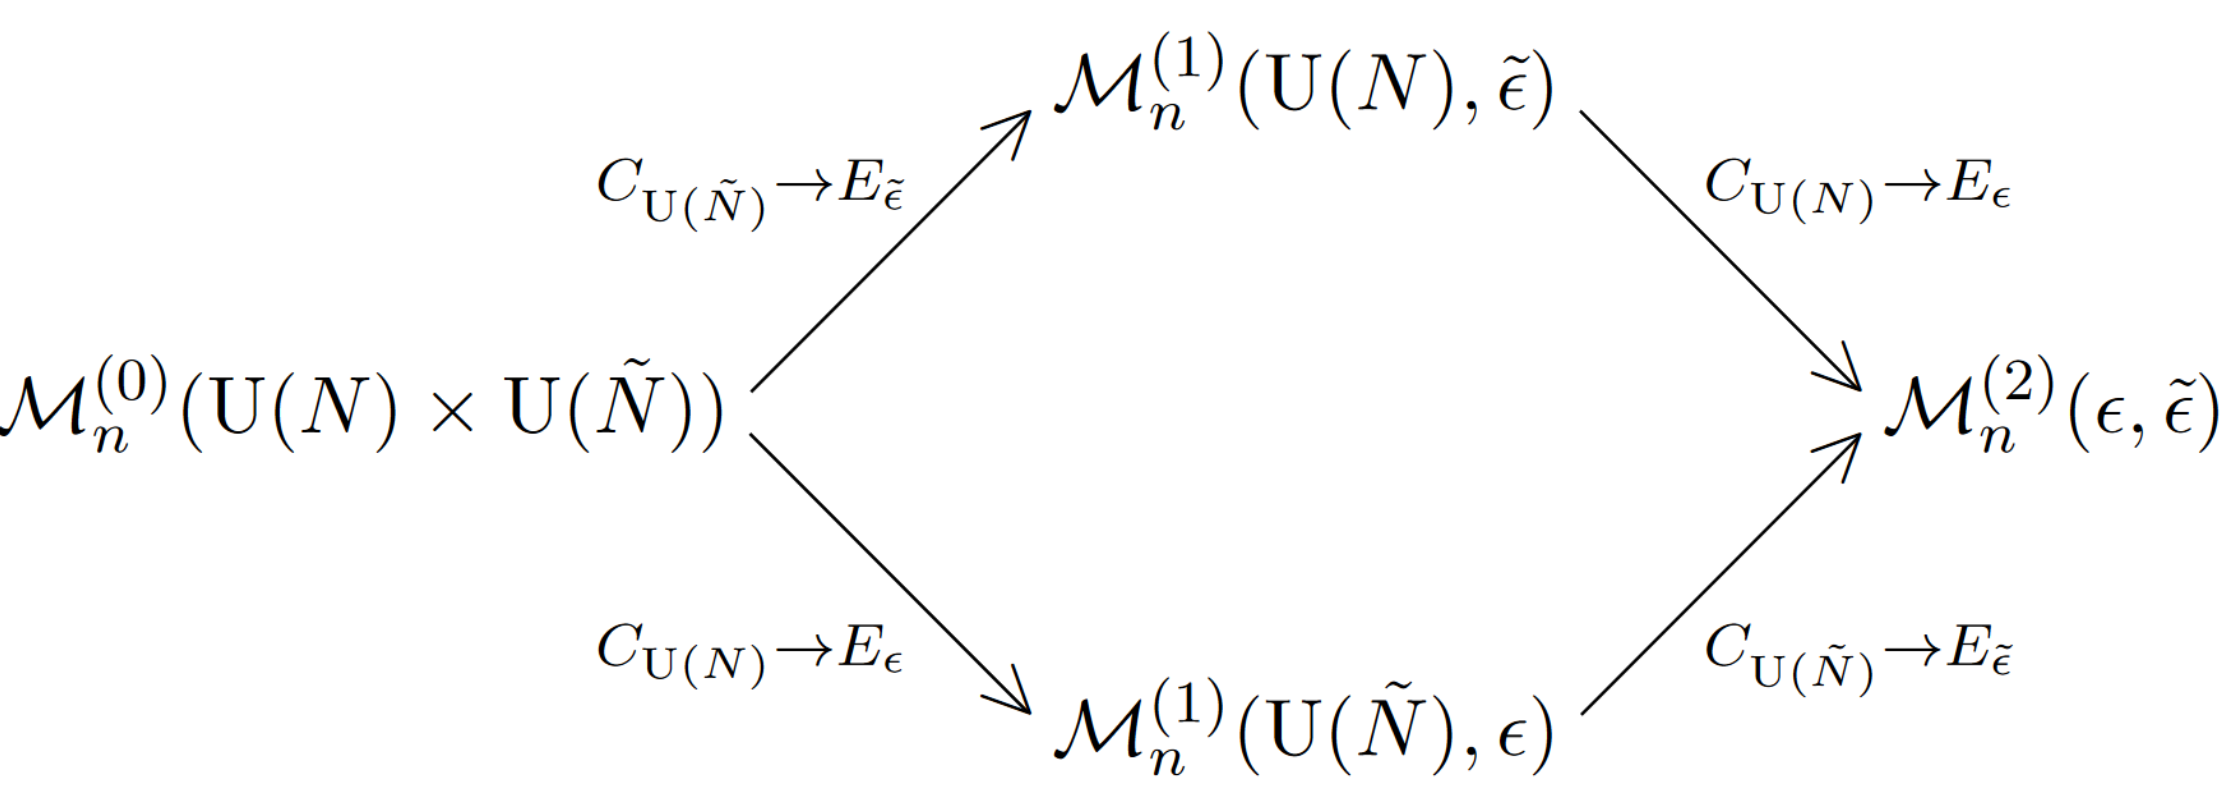
\includegraphics[width=1\linewidth]{main.png}
    \end{figure}
\end{frame}
\begin{frame}
    \frametitle{Double partial amplitudes}
    Because there are two color indices in this sclar theory, so it can be anticipateed that the amplitude
    have double trace decomposition structure
    \begin{align*}
        \mathcal{M}_n^{(0)}&=\sum_{\alpha\in S_n/Z_n}\mathrm{Tr}(\tilde{T}^{\mathsf{b}_{\alpha(1)}}\tilde{T}^{\mathsf{b}_{\alpha(2)}}\cdots\tilde{T}^{\mathsf{b}_{\alpha(n)}})M_n^{(0)}(\alpha(1),\alpha(2),\ldots,\alpha(n))\\
        &=\sum_{\alpha,\beta\in S_n/Z_n}\mathrm{Tr}(\tilde{T}^{\mathsf{b}_{\alpha(1)}}\tilde{T}^{\mathsf{b}_{\alpha(2)}}\cdots\tilde{T}^{\mathsf{b}_{\alpha(n)}})\text{Tr}(T^{\mathtt{a}_{\beta(1)}}T^{\mathtt{a}_{\beta(2)}}\cdots T^{\mathtt{a}_{\beta(n)}})\\
        &\times \alert{m_n^{(0)}(\alpha|\beta)}
    \end{align*} 
    where the last term $m_n^{(0)}(\alpha|\beta)$ is called \alert{double partial amplitude} and can be read off from the full amplitude
    \begin{align*}
    m_{n}^{(0)}(\alpha|\beta)&=\int\frac{d^{n}\sigma}{\operatorname{vol}\operatorname{SL}(2,\mathbb{C})}\frac{\prod_{a}{}^{\prime}\delta(\sum_{b\neq a}\frac{s_{ab}}{\sigma_{ab}})}{(\sigma_{\alpha(1),\alpha(2)}\cdots\sigma_{\alpha(n),\alpha(1)})(\sigma_{\beta(1),\beta(2)}\cdots\sigma_{\beta(n),\beta(1)})}\\
    =&\sum_{\{\sigma\}\in\mathrm{solutions}}\frac1{\det^{\prime}\Phi}\frac{1}{(\sigma_{\alpha(1),\alpha(2)}\cdots\sigma_{\alpha(n),\alpha(1)})(\sigma_{\beta(1),\beta(2)}\cdots\sigma_{\beta(n),\beta(1)})}
    \end{align*}

\end{frame}
\begin{frame}
    Likewise the decomposition in the first section, it is more usually to write the amplitudes in terms of colore basis
    \begin{equation*}
        \boxed{\mathbf{c}_\alpha\equiv\sum_{\mathsf{c}_1,...,\mathsf{c}_{n-3}}f_{\mathsf{a}_1\mathsf{a}_{\alpha(2)}\mathsf{c}_1}\cdots f_{\mathsf{c}_{n-3}\mathsf{a}_{\alpha(n-1)}\mathsf{a}_n}}
    \end{equation*}
    where $\alpha \in S_{n-2}$. The amplitude is 
    \begin{equation*}
        \mathcal{M}_n^{(0)}=\sum_{\alpha,\beta\in S_{n-2}}\mathbf{c_\alpha}\tilde{\mathbf{c_\beta}}m_{n}^{(0)}(\alpha|\beta)
    \end{equation*}
\end{frame}
\begin{frame}
    \frametitle{Examples}
    \begin{itemize}
        \item The simplest example is the 3 point case
        \begin{equation*}
            \mathcal{M}_3^{(0)}(1^{aa^\prime,bb^\prime,cc^\prime})=(\sigma_{12}\sigma_{23}\sigma_{31})^2\frac{f_{abc}f_{a^\prime b^\prime c^\prime}}{(\sigma_{12}\sigma_{23}\sigma_{31})^2}=f_{abc}f_{a^\prime b^\prime c^\prime}
        \end{equation*}
        It actually gives the correct answer.
        \item The 4 point case is a little complex. Solving the scattering equations with $\sigma_1=0,\sigma_2=1,\sigma_3=\infty$ gives $\sigma_4=-s_{23}/s_{12}$. Define
        $s_{12}=s$, $s_{23}=t$, $s_{13}=u$, the color factors are 
        \begin{equation*}
            \mathbf{c_s}=\sum_bf_{a_1a_2b}f_{ba_3a_4},\mathbf{c_t}=\sum_bf_{a_1a_4b}f_{ba_3a_2},\mathbf{c_u}=\sum_bf_{a_1a_3b}f_{ba_2a_4}
        \end{equation*}
        Denoting the ordering $(1324)$ as $P$ and comuputing $\det{'}\Phi=\frac{s^2}{t}/(\sigma_{12}\sigma_{23}^2\sigma_{31}\sigma_{34}\sigma_{42})$, one gets
    \end{itemize}
\end{frame}
\begin{frame}
    \begin{align*}
        \!\!\!\!\mathcal{M}_4^{(0)}&=\mathbf{c_s}\tilde{\mathbf{c_s}}m_4^{(0)}(I;I)+\mathbf{c_s}\tilde{\mathbf{c_u}}m_4^{(0)}(I;P)+\mathbf{c_u}\tilde{\mathbf{c_s}}m_4^{(0)}(P;I)+\mathbf{c_u}\tilde{\mathbf{c_u}}m_4^{(0)}(P;P)\\
        &=\mathbf{c_s}\tilde{\mathbf{c_s}}\frac{u}{st}+(\mathbf{c_s}\tilde{\mathbf{c_u}}+\mathbf{c_u}\tilde{\mathbf{c_s}})\frac{1}{t}+\mathbf{c_u}\tilde{\mathbf{c_u}}\frac{s}{ut}\\
        &=-\frac{\mathbf{c_s}\tilde{\mathbf{c_s}}}{s}-\frac{\mathbf{c_t}\tilde{\mathbf{c_t}}}{t}-\frac{\mathbf{c_u}\tilde{\mathbf{c_u}}}{u}
    \end{align*}
    \quad \quad as expected for a color-dressed cubic theory.
    \begin{itemize}
        \item For the five point, I just give the results of some double partial amplitudes.
        Denoting the orderings as $I=P_0$, $(13245)=P_1$, $(12435)=P_2$, $(14325)=P_3$, $(13425)=P_4$, $(14235)=P_5$
        \begin{equation*}
            \begin{aligned}&m_5^{(0)}(I|I)=\frac{1}{s_{12}s_{34}}+\frac{1}{s_{23}s_{45}}+\frac{1}{s_{34}s_{51}}+\frac{1}{s_{45}s_{12}}+\frac{1}{s_{51}s_{23}},\\&m_5^{(0)}(I|P_1)=-\frac{1}{s_{23}}\left(\frac{1}{s_{45}}+\frac{1}{s_{12}}\right),\quad
                m_5^{(0)}(I|P_2)=-\frac{1}{s_{34}}\left(\frac{1}{s_{51}}+\frac{1}{s_{12}}\right).\end{aligned}
        \end{equation*}
    \end{itemize}
\end{frame}
\begin{frame}
    \begin{align*}
        &m_5^{(0)}(I|P_3)=-\frac{1}{s_{51}}\left(\frac{1}{s_{23}}+\frac{1}{s_{34}}\right),\quad  m_5^{(0)}(I|P_4)=-\frac{1}{s_{34}s_{51}},\\
        &m_5^{(0)}(I|P_5)=0
    \end{align*}
    From there examples, it is easy to see that when both permutations in $m_n^{(0)}(\alpha|\beta)$ are the same, then the answer is a sum over all color-orded
    trivalent diagrams; When the two permutations are different, it gives a subset of terms of $m_n^{(0)}(\alpha|\alpha)$. 
    \\ \hspace*{\fill}\\
    More explicitly,


    \tikzset{every picture/.style={line width=0.75pt}} %set default line width to 0.75pt        

    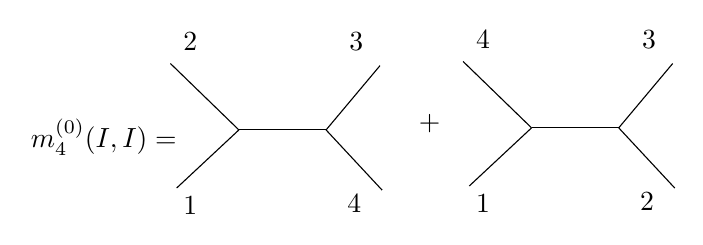
\begin{tikzpicture}[x=0.75pt,y=0.75pt,yscale=-1,xscale=1]
    %uncomment if require: \path (0,300); %set diagram left start at 0, and has height of 300
    
    %Straight Lines [id:da8455657796938298] 
    \draw    (179.5,110) -- (212.5,142) ;
    %Straight Lines [id:da5324594211620186] 
    \draw    (212.5,142) -- (182.5,170) ;
    %Straight Lines [id:da4643902351443361] 
    \draw    (212.5,142) -- (254.5,142) ;
    %Straight Lines [id:da8904360433186445] 
    \draw    (280.5,111) -- (254.5,142) ;
    %Straight Lines [id:da18000644921445508] 
    \draw    (254.5,142) -- (281.5,171) ;
    %Straight Lines [id:da29602344087941934] 
    \draw    (320.5,109) -- (353.5,141) ;
    %Straight Lines [id:da9975053882839713] 
    \draw    (353.5,141) -- (323.5,169) ;
    %Straight Lines [id:da5157442319090852] 
    \draw    (353.5,141) -- (395.5,141) ;
    %Straight Lines [id:da049884375007126946] 
    \draw    (421.5,110) -- (395.5,141) ;
    %Straight Lines [id:da9299487354359295] 
    \draw    (395.5,141) -- (422.5,170) ;
    
    % Text Node
    \draw (111,135.4) node [anchor=north west][inner sep=0.75pt]    {$m_{4}^{(0)}(I,I) =$};
    % Text Node
    \draw (184.5,173) node [anchor=north west][inner sep=0.75pt]   [align=left] {1};
    % Text Node
    \draw (184.5,94) node [anchor=north west][inner sep=0.75pt]   [align=left] {2};
    % Text Node
    \draw (264.5,94) node [anchor=north west][inner sep=0.75pt]   [align=left] {3};
    % Text Node
    \draw (263.5,172) node [anchor=north west][inner sep=0.75pt]   [align=left] {4};
    % Text Node
    \draw (298,133.4) node [anchor=north west][inner sep=0.75pt]    {$+$};
    % Text Node
    \draw (325.5,172) node [anchor=north west][inner sep=0.75pt]   [align=left] {1};
    % Text Node
    \draw (325.5,93) node [anchor=north west][inner sep=0.75pt]   [align=left] {4};
    % Text Node
    \draw (405.5,93) node [anchor=north west][inner sep=0.75pt]   [align=left] {3};
    % Text Node
    \draw (404.5,171) node [anchor=north west][inner sep=0.75pt]   [align=left] {2};
    
    
    \end{tikzpicture}

\end{frame}
\begin{frame}
    Similarly,
    


    \tikzset{every picture/.style={line width=0.75pt}} %set default line width to 0.75pt        

    \begin{tikzpicture}[x=0.75pt,y=0.75pt,yscale=-1,xscale=1]
    %uncomment if require: \path (0,350); %set diagram left start at 0, and has height of 350
    
    %Straight Lines [id:da8963901965951664] 
    \draw    (84,71) -- (108,93) ;
    %Straight Lines [id:da07470927432540231] 
    \draw    (108,93) -- (136,93) ;
    %Straight Lines [id:da12245379377221366] 
    \draw    (108,93) -- (85,111) ;
    %Straight Lines [id:da6511432990080723] 
    \draw    (136,93) -- (161,114) ;
    %Straight Lines [id:da1430135957918477] 
    \draw    (157,71) -- (136,93) ;
    %Straight Lines [id:da8765002291973463] 
    \draw    (157,71) -- (158,47) ;
    %Straight Lines [id:da9623971067643409] 
    \draw    (157,71) -- (178,87) ;
    %Straight Lines [id:da5561877649988292] 
    \draw    (214,70) -- (238,92) ;
    %Straight Lines [id:da44100018812085007] 
    \draw    (238,92) -- (266,92) ;
    %Straight Lines [id:da05824517478761182] 
    \draw    (238,92) -- (215,110) ;
    %Straight Lines [id:da35334338456014613] 
    \draw    (266,92) -- (291,113) ;
    %Straight Lines [id:da9313767826880515] 
    \draw    (287,70) -- (266,92) ;
    %Straight Lines [id:da696534040519218] 
    \draw    (287,70) -- (288,46) ;
    %Straight Lines [id:da5526828548209644] 
    \draw    (287,70) -- (308,86) ;
    %Straight Lines [id:da19124382298581288] 
    \draw    (359,64) -- (383,86) ;
    %Straight Lines [id:da5237814153432139] 
    \draw    (383,86) -- (411,86) ;
    %Straight Lines [id:da7974585866426673] 
    \draw    (383,86) -- (360,104) ;
    %Straight Lines [id:da46316924534551385] 
    \draw    (411,86) -- (436,107) ;
    %Straight Lines [id:da37617479030606993] 
    \draw    (432,64) -- (411,86) ;
    %Straight Lines [id:da9834219129393018] 
    \draw    (432,64) -- (433,40) ;
    %Straight Lines [id:da7117622111604034] 
    \draw    (432,64) -- (453,80) ;
    %Straight Lines [id:da8760088009181417] 
    \draw    (82,171) -- (106,193) ;
    %Straight Lines [id:da7078786925271212] 
    \draw    (106,193) -- (134,193) ;
    %Straight Lines [id:da5389180018159456] 
    \draw    (106,193) -- (83,211) ;
    %Straight Lines [id:da26578622720899636] 
    \draw    (134,193) -- (159,214) ;
    %Straight Lines [id:da5989066756692625] 
    \draw    (155,171) -- (134,193) ;
    %Straight Lines [id:da13747441694892726] 
    \draw    (155,171) -- (156,147) ;
    %Straight Lines [id:da4119117050779677] 
    \draw    (155,171) -- (176,187) ;
    %Straight Lines [id:da5379584617019675] 
    \draw    (221,169) -- (245,191) ;
    %Straight Lines [id:da788296500370655] 
    \draw    (245,191) -- (273,191) ;
    %Straight Lines [id:da4136462405421193] 
    \draw    (245,191) -- (222,209) ;
    %Straight Lines [id:da37414431568833373] 
    \draw    (273,191) -- (298,212) ;
    %Straight Lines [id:da8232480161298765] 
    \draw    (294,169) -- (273,191) ;
    %Straight Lines [id:da7983669347123197] 
    \draw    (294,169) -- (295,145) ;
    %Straight Lines [id:da7903324165137171] 
    \draw    (294,169) -- (315,185) ;
    
    % Text Node
    \draw (5,76.4) node [anchor=north west][inner sep=0.75pt]    {$m_{5}( I,I) =$};
    % Text Node
    \draw (87,114) node [anchor=north west][inner sep=0.75pt]   [align=left] {1};
    % Text Node
    \draw (86,68) node [anchor=south west] [inner sep=0.75pt]   [align=left] {2};
    % Text Node
    \draw (159.5,56) node [anchor=south west] [inner sep=0.75pt]   [align=left] {3};
    % Text Node
    \draw (180,84) node [anchor=south west] [inner sep=0.75pt]   [align=left] {4};
    % Text Node
    \draw (163,111) node [anchor=south west] [inner sep=0.75pt]   [align=left] {5};
    % Text Node
    \draw (198,73.4) node [anchor=north west][inner sep=0.75pt]    {$+$};
    % Text Node
    \draw (217,113) node [anchor=north west][inner sep=0.75pt]   [align=left] {2};
    % Text Node
    \draw (216,67) node [anchor=south west] [inner sep=0.75pt]   [align=left] {3};
    % Text Node
    \draw (289.5,55) node [anchor=south west] [inner sep=0.75pt]   [align=left] {4};
    % Text Node
    \draw (310,83) node [anchor=south west] [inner sep=0.75pt]   [align=left] {5};
    % Text Node
    \draw (293,110) node [anchor=south west] [inner sep=0.75pt]   [align=left] {1};
    % Text Node
    \draw (335,72.4) node [anchor=north west][inner sep=0.75pt]    {$+$};
    % Text Node
    \draw (362,107) node [anchor=north west][inner sep=0.75pt]   [align=left] {3};
    % Text Node
    \draw (361,61) node [anchor=south west] [inner sep=0.75pt]   [align=left] {4};
    % Text Node
    \draw (434.5,49) node [anchor=south west] [inner sep=0.75pt]   [align=left] {5};
    % Text Node
    \draw (455,77) node [anchor=south west] [inner sep=0.75pt]   [align=left] {1};
    % Text Node
    \draw (438,104) node [anchor=south west] [inner sep=0.75pt]   [align=left] {2};
    % Text Node
    \draw (65,184.4) node [anchor=north west][inner sep=0.75pt]    {$+$};
    % Text Node
    \draw (85,214) node [anchor=north west][inner sep=0.75pt]   [align=left] {4};
    % Text Node
    \draw (84,168) node [anchor=south west] [inner sep=0.75pt]   [align=left] {5};
    % Text Node
    \draw (157.5,156) node [anchor=south west] [inner sep=0.75pt]   [align=left] {1};
    % Text Node
    \draw (178,184) node [anchor=south west] [inner sep=0.75pt]   [align=left] {2};
    % Text Node
    \draw (161,211) node [anchor=south west] [inner sep=0.75pt]   [align=left] {3};
    % Text Node
    \draw (201,181.4) node [anchor=north west][inner sep=0.75pt]    {$+$};
    % Text Node
    \draw (224,212) node [anchor=north west][inner sep=0.75pt]   [align=left] {5};
    % Text Node
    \draw (226,172) node [anchor=south west] [inner sep=0.75pt]   [align=left] {1};
    % Text Node
    \draw (296.5,154) node [anchor=south west] [inner sep=0.75pt]   [align=left] {2};
    % Text Node
    \draw (317,182) node [anchor=south west] [inner sep=0.75pt]   [align=left] {3};
    % Text Node
    \draw (300,209) node [anchor=south west] [inner sep=0.75pt]   [align=left] {4};
    
    
    \end{tikzpicture}
\end{frame}
\begin{frame}
    \frametitle{Trivalent graph expansion}
    \begin{alertblock}{Proposition}
        The function $m_n^{(0)}(\alpha|\beta)$ computes the sum of all trivalent scalar diagrams which can be regarded as both $\alpha$ color-ordered and $\beta$ color-orded.
    \end{alertblock}
    \pause
    More explicitly, 
    \begin{equation*}
        \boxed{m_n^{(0)}(\alpha|\beta)=(-1)^{n-3+n_{\text{flip}}(\alpha|\beta)}\sum_{g\in\mathcal{T}(\alpha)\cap\mathcal{T}(\beta)}\prod_{e\in E(g)}\frac{1}{s_e}}
\end{equation*}
where the $\text{flip}(\alpha|\beta)$ is defined below, $\mathcal{T}(\alpha)$ and $\mathcal{T}(\beta)$ refer to the set of color-ordered diagrams in $\alpha$ and 
$\beta$ ordering respectively. To make this expression more clear, see the following diagram
\begin{figure}[htb]
    \centering
    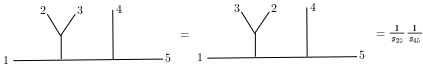
\includegraphics[width=0.8\linewidth]{5.png}
\end{figure}
\end{frame}
\begin{frame}
    We take $m_8^{(0)}(I;18543762)$ as an example to explain how to compute it in an systematic way
    \begin{itemize}
        \item First step, draw a disk with n nodes sitting on the boundary in the ordering $\alpha$, then link the n nodes with a loop of line segments according to
              the ording $\beta$. The line segments from $\beta$ split the disk into some polygons, like the graph (b). We need to move the external points of every polygon
              to make them have no common edges, like graph (c).
        \item Second step, put a point in every polygon, named equivalant vertex, and connect this point to all external points in corresponding area. Lines that connect equivalent 
              vertices in two regions with common vertices are called equivalent propagators. The resulting graph is an equivalent Feynman diagram, as shown in Figure (d).
    \end{itemize}
\end{frame}
\begin{frame}
    \begin{itemize}
        \item Third step, we can read off the corresponding amplitudes from the equivalent Feynman diagram. 
    \end{itemize}
    \begin{figure}
        \centering
        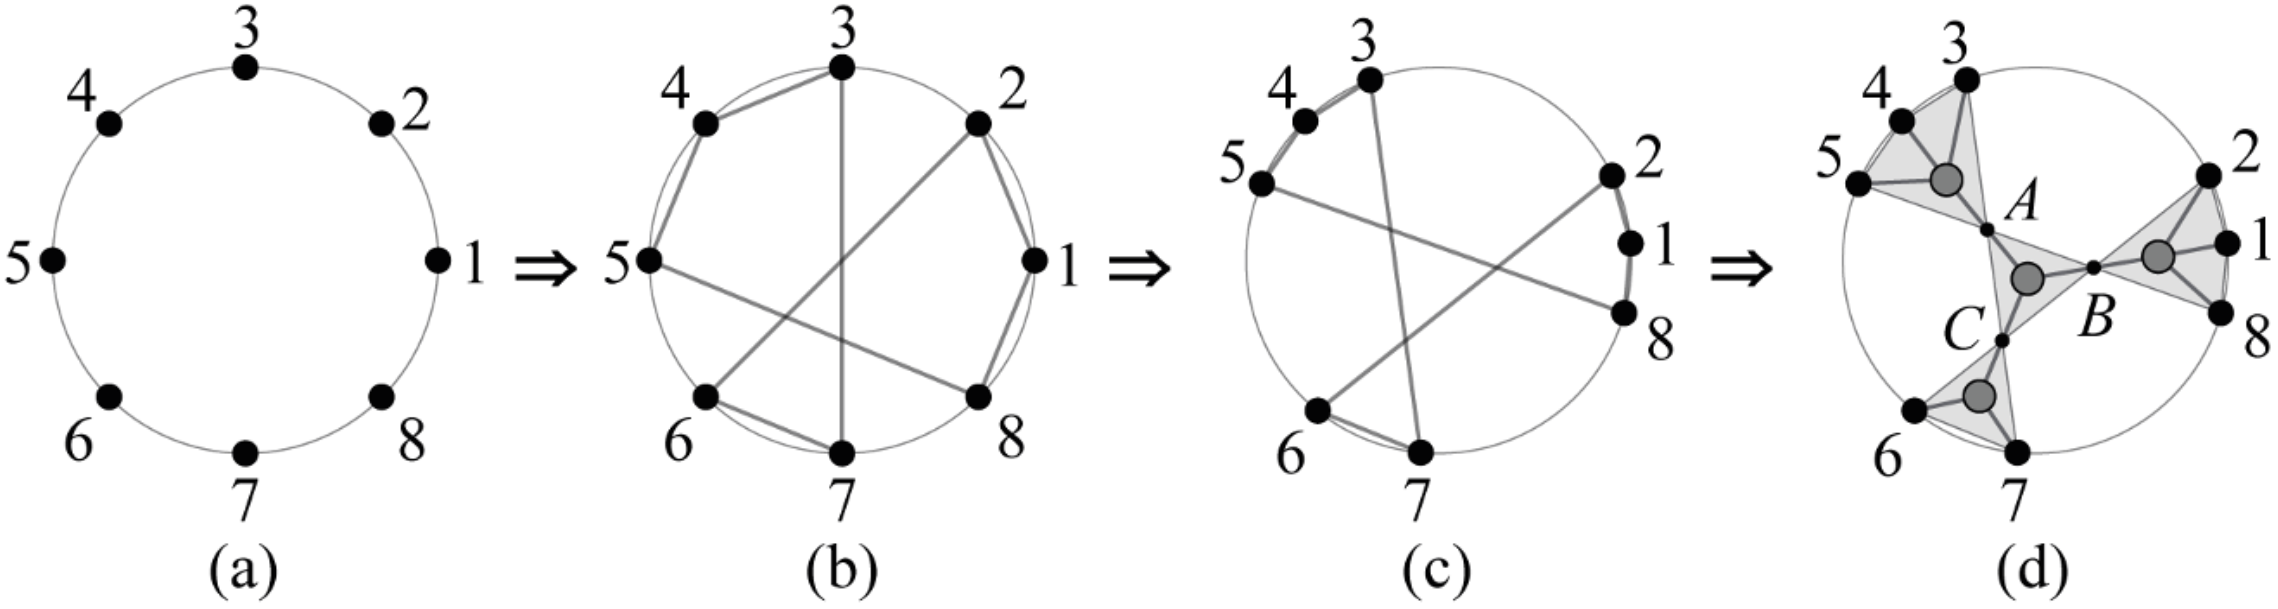
\includegraphics[width=1\linewidth]{7.png}
    \end{figure}
    In this example, we can obtain 
    \begin{equation*}
        m_8^{(0)}(I|54376218)=(-1)^?\left(\frac{1}{s_{21}}+\frac{1}{s_{18}}\right)\left(\frac{1}{s_{34}}+\frac{1}{s_{45}}\right)\frac{1}{s_{345}s_{812}s_{67}}
    \end{equation*}
    As for the indefinite sign, there is also a procedure to determine it.
\end{frame}
\begin{frame}
    \begin{itemize}
        \item First step, determine the orientation of the disk by ordering $\alpha$, and define the loop segments by ordering $\beta$, which also determine the orientation of every polygon.
        \item Second step, (1) each polygon with odd number vertices contributes a plus sign if the orientation is the same as disk, and a minus sign oppositely;
              (2) each polygon with even number vertices contribute a minus sign; (3) each intersection point contributes a minus sign.
    \end{itemize}
    \begin{figure}
        \centering
        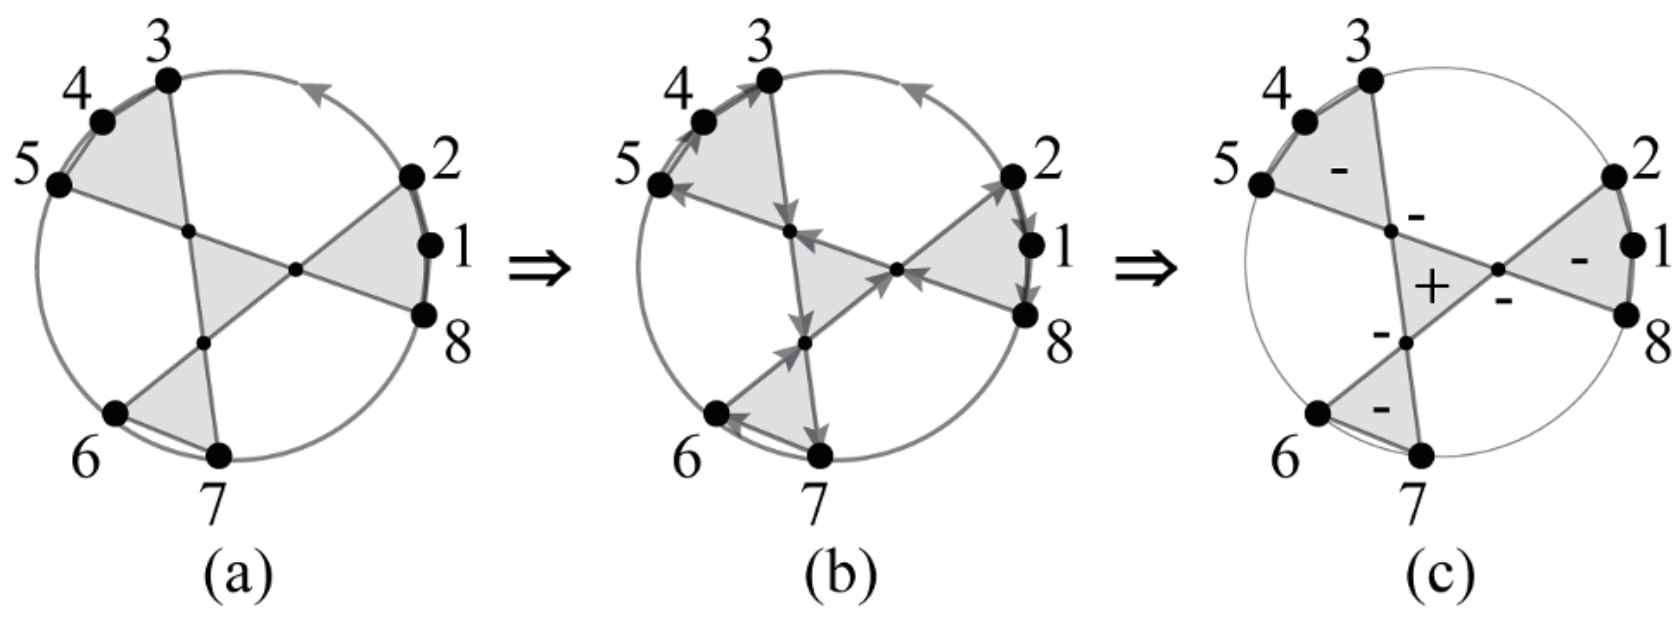
\includegraphics[width=1\linewidth]{6.png}
    \end{figure}
\end{frame}
\begin{frame}
    \frametitle{Relation to KLT matrix}
    It can be shown that the scalar double partial amplitudes are the same as the inverse of KLT matrix.
    \begin{align*}
        &(S_{\mathrm{KLT}}^{-1})_\beta^\alpha=(m_{\mathrm{scalar}})_\beta^\alpha\\
        &\equiv m^{(0)}(1,\alpha(2),\ldots,\alpha(n-2),n-1,n|1,\beta(2),\ldots,\beta(n-2),n,n-1)
    \end{align*}
    The inverse of KLT matrix have been also discussed in other paper, in which it was related to field theory limit if string 
    disk integrals, so it would be interesting to explore the connection further. 
\end{frame}
\begin{frame}
    \frametitle{Color-Kinematics Duality again}
    At the begining, I mentioned that sclar-, gluon- and graviton- amplitudes can be related by simple transformations ($C\to E$ or $\tilde{C}\to\tilde{E}$ or both).
    More explicitly,
    \begin{equation*}
        {\cal M}^{(0)}_n =\!\!\sum_{I=1}^{(n-3)!}\frac{C(\sigma^{(I)}){\tilde C}(\sigma^{(I)})}{{\rm det}'\Phi(\sigma^{(I)})},\quad {\cal M}^{(1)}_n = \!\!\sum_{I=1}^{(n-3)!}\frac{C(\sigma^{(I)}){\tilde E}(\sigma^{(I)})}{{\rm det}'\Phi(\sigma^{(I)})},
    \end{equation*}
    \begin{equation*}
        {\cal M}^{(2)}_n = \!\!\sum_{I=1}^{(n-3)!}\frac{E(\sigma^{(I)}){\tilde E}(\sigma^{(I)})}{{\rm det}'\Phi(\sigma^{(I)})}.
    \end{equation*}
    If we expand the color factor like 
    \begin{equation*}
        C=\sum_{\gamma\in S_{n-2}}\frac{{\bf c}_{1\gamma(2)\cdots\gamma(n-1)n}}{\sigma_{1,\gamma(2)}\cdots\sigma_{\gamma(n-1),n}\sigma_{n,1}},
    \end{equation*}
\end{frame}
\begin{frame}
    It hints the exsitence of similar form for $E$. More explicitly, there must functions, denoted as $\boldsymbol{n}$, which depends only on kinematic data $\{\epsilon^{\mu}_a,k^\mu_a \}$
    \begin{equation*}
        E = {\rm Pf}'\Psi(\epsilon,k,\sigma ) = \sum_{\gamma\in S_{n-2}}\frac{{\bf n}_{1\gamma(2)\cdots\gamma(n-1)n}}{\sigma_{1,\gamma(2)}\cdots\sigma_{\gamma(n-1),n}\sigma_{n,1}}.
    \end{equation*}
    Now we can unify $\bf c$ and $\bf n$ as e in all three theories, the full amplitude can be written in a unified form
    \begin{equation*}
       \mathcal{M}_n^{(s)}=\sum_{\alpha,\beta\in S_{n-2}}e_\alpha e_\beta m^{(0)}(\alpha|\beta)
    \end{equation*}
    and the factor satisfies the "BCJ" relation
    \begin{equation*}
        e_{g_t}=\pm(e_{g_s}-e_{g_u})
    \end{equation*}
    If we contentate on pure Yang-Mills theory, the realtion is just the one we list in the first second section.
\end{frame}
\end{document}


